%% Template basiert auf der Vorlage der Uni Graz für VWA: https://latex.tugraz.at/vorlagen/allgemein

%% Versionen:
%% V1: 9. Augugst 2021 (GreiA)



%% %%%%%%%%%%%%%%%%%%%%%%%%%%%%%%%%%%%%%%%%%%%%%%%%%%%%%%%%%%%%%%%%%%%
%% Allgemeine Festlegungen für die Darstellung des Gesamtdokumentes;
%% %%%%%%%%%%%%%%%%%%%%%%%%%%%%%%%%%%%%%%%%%%%%%%%%%%%%%%%%%%%%%%%%%%%
\newcommand{\mypapersize}{A4}
%% e.g., "A4", "letter", "legal", "executive", ...
%% The size of the paper of the resulting PDF file.

\newcommand{\mylaterality}{twoside}
%% "oneside" or "twoside"
%% Either you are creating a document which is printed on both, left pages
%% and right pages (twoside) or you create a document which is printed
%% on right pages only (oneside).

\newcommand{\mydraft}{false}
%% "true" or "false"
%% Use draft mode? If true, included graphics are replaced by empty
%% rectangles (of same size) and overfull boxes (in margin space) are
%% marked with black box (-> easy to spot!)

\newcommand{\myparskip}{half}
%% e.g., "no", "full", "half", ...
%% How to separate paragraphs: indention ("no") or spacing ("half",
%% "full", ...).

\newcommand{\myBCOR}{0mm}
%% Inner binding correction. This value depends on the method which is
%% being used to bind your printed result. Some techniques do not
%% require a binding correction at all ("0mm"), other require for
%% example "5mm". Refer to KOMA script documentation for a detailed
%% explanation what a binding correction is and how to measure it.

\newcommand{\myfontsize}{12pt}
%% e.g., 10pt, 11pt, 12pt
%% The font size of the main text in pt (points).

\newcommand{\mylinespread}{1.0}
%% e.g., 1.0, 1.5, 2.0
%% Line spacing in %/100. For example 1.5 means 150% of the usual line
%% spacing. Please use with caution: 100% ("1.0") is fine because the
%% font was designed for it.

\newcommand{\mylanguage}{american,ngerman}
%% "english,ngerman", "ngerman,english", ...
%% NOTE: The *last* language is the active one!
%% See babel documentation for further details.

%% BibLaTeX-settings: (see biblatex reference for further description)
\newcommand{\mybiblatexstyle}{authoryear}
%% e.g., "alphabetic", "authoryear", ...
%% The biblatex style which is being used for referencing. See
%% biblatex documentation for further details and more values.
%%
%% CAUTION: if you change the style, please check for (in)compatible
%%          "biblatex" package options in the file
%%          "template/preamble.tex"! For example: "alphabetic" does
%%          not have an option "dashed=..." and causes an error if it
%%          does not get removed from the list of options.

\newcommand{\mybiblatexdashed}{false}  %% "true" or "false"
%% If true: replace recurring reference authors with a dash.

\newcommand{\mybiblatexbackref}{true}  %% "true" or "false"
%% If true: create backward links from reference to citations.

\newcommand{\mybiblatexfile}{references-biblatex.bib}
%% Name of the biblatex file that holds the references.

\newcommand{\mydispositioncolor}{30,103,182}
%% e.g., "30,103,182" (blue/turquois), "0,0,0" (black), ...
%% Color of the headings and so forth in RGB (red,green,blue) values.
%% NOTE: if you are using "0,0,0" for black, printers might still
%%       recognize pages as color pages. In case this is a problem
%%       (paying for color print-outs vs. paying for b/w-printouts)
%%       please edit file "template/preamble.tex" and change
%%       "\definecolor{DispositionColor}{RGB}{\mydispositioncolor}"
%%       to "\definecolor{DispositionColor}{gray}{0}" and thus
%%       overwriting the value of \mydispositioncolor above.

\newcommand{\mycolorlinks}{true}  %% "true" or "false"
%% Enables or disables colored links (hyperref package).



\newcommand{\mytitlepage}{template/title_thesis_htlinn} %Titelseite

\newcommand{\mytodonotesoptions}{}
%% e.g., "" (empty), "disable", ...
%% Options for the todonotes-package. If "disable", all todonotes will
%% be hidden (including listoftodos).

%% Load main settings for document preamble:
\documentclass[%
fontsize=\myfontsize,%% size of the main text
paper=\mypapersize,  %% paper format
parskip=\myparskip,  %% vertical space between paragraphs (instead of indenting first par-line)
DIV=calc,            %% calculates a good DIV value for type area; 66 characters/line is great
headinclude=true,    %% is header part of margin space or part of page content?
footinclude=false,   %% is footer part of margin space or part of page content?
open=right,          %% "right" or "left": start new chapter on right or left page
appendixprefix=true, %% adds appendix prefix; only for book-classes with \backmatter
bibliography=totoc,  %% adds the bibliography to table of contents (without number)
draft=\mydraft,      %% if true: included graphics are omitted and black boxes
                     %%          mark overfull boxes in margin space
BCOR=\myBCOR,        %% binding correction (depends on how you bind
                     %% the resulting printout.
\mylaterality        %% oneside: document is not printed on left and right sides, only right side
                     %% twoside: document is printed on left and right sides
]{scrbook}  %% article class of KOMA: "scrartcl", "scrreprt", or "scrbook".
            %% CAUTION: If documentclass will be changed, *many* other things
            %%          change as well like heading structure, ...

\usepackage{float}
\usepackage{ifthen}
\usepackage[T1]{fontenc}
\usepackage{lmodern}
\usepackage[utf8]{inputenc} %% UTF8 as input characters
\usepackage{textcomp}
\usepackage[\mylanguage]{babel}  %% used languages; default language is *last* language of options
\usepackage{scrlayer-scrpage} %%  advanced page style using KOMA


\ifthenelse{\boolean{\mydraft}}{   %% the \mydraft switches between
                                   %% showing rectangles instead of graphics
  \usepackage[pdftex,draft]{graphicx}
}
{
  \usepackage[pdftex]{graphicx}
}

\usepackage{pifont}
%% pre-define ifthen-boolean variables:
\newboolean{myaddcolophon}
\newboolean{myaddlistoftodos}
\newboolean{english_affidavit}
\usepackage{xspace}
\usepackage[usenames,dvipsnames]{xcolor}
\definecolor{DispositionColor}{RGB}{\mydispositioncolor} %% used for links and so forth in screen-version

\usepackage[normalem]{ulem}
\usepackage{framed}
\usepackage{eso-pic}
\usepackage{enumitem}
\usepackage[\mytodonotesoptions]{todonotes}  %% option "disable" removes all todonotes output from 
\usepackage{units}
\usepackage{listings}
%% DO NOT REMOVE THIS LINE!

\setboolean{myaddcolophon}{true}  %% "true" or "false"
%% If set to "true": a colophon (with notes about this document
%% template, LaTeX, ...) is added after the title page.
%% Please do not set to "false" without a good reason. The colophon
%% helps your readers to get in touch with LaTeX and to find this template.

\setboolean{myaddlistoftodos}{false}  %% "true" or "false"
%% If set to "true": the current list of open todos is added after the
%% table of contents. If \mytodonotesoptions is set to "disable", no
%% list of todos is added, independent of this setting here.

\setboolean{english_affidavit}{true}  %% "true" or "false"
%% If set to "true": the language of the statutory declaration text is set to
%% English, otherwise it is in German.




%% ========================================================================
%% Document metadata: DIESE WERTE BITTE ANPASSEN, wie werden dann automatisch auf der
%% Titelseite angezeigt
%% ========================================================================

\newcommand{\myprojectpartner}{HTL Anichstraße} 
\newcommand{\mytitle}{Artificial Intelligence in the Industry and Education Environment} %% Titel der Arbeit
\newcommand{\mysubtitle}{SUBTITITLE}
\newcommand{\myinstitute}{Abteilung für Wirtschaftsingenieure/Betriebsinformatik} 
\newcommand{\mysubmissionyear}{2025} %% Einreich - Jahr
\newcommand{\mysubmissionmonth}{April} %% Monat der Einreichung
\newcommand{\myauthor}{Gabriel Mrkonja\\Florian Prandstetter\\Luna Schätzle}  %% Autoren. Bitte mit \\ Trennen wenn mehrere
\newcommand{\mysupervisor}{Greinöcker\\Egger}  %%Betreuer. Bitte mit \\ Trennen wenn mehrere
%%\newcommand{\myprojectpartner}{Vollständige Bezeichnung der Firma}  %% Partnerfirma

\newcommand{\mysubject}{SUBJECT}  %% also used for PDF metadata (hyperref)
\newcommand{\mykeywords}{KEYWORDS}  %% also used for PDF metadata (hyperref)


%% header settings
\usepackage{lastpage}

\ohead{\headmark }
\ihead*{
\includegraphics[width=3cm]{figures/htl-logo}}

\ifoot{\thepage}  %Will man Anzahl Seiten: /\pageref{LastPage}
\ofoot{\myauthor}


%% ========================================================================
%%%% MISC command definitions
%% ========================================================================
%% Time-stamp: <2015-04-30 17:19:58 vk>
%%%% === Disclaimer: =======================================================
%% created by
%%
%%      Karl Voit
%%
%% using GNU/Linux, GNU Emacs & LaTeX 2e
%%

%doc%
%doc% \section{\texttt{mycommands.tex} --- various definitions}\myinteresting
%doc% \label{sec:mycommands}
%doc%
%doc% In file \verb#template/mycommands.tex# many useful commands are being
%doc% defined. 
%doc% 
%doc% \paragraph{What should I do with this file?} Please take a look at its 
%doc% content to get the most out of your document.
%doc% 

%doc% 
%doc% One of the best advantages of \LaTeX{} compared to \myacro{WYSIWYG} software products is
%doc% the possibility to define and use macros within text. This empowers the user to
%doc% a great extend.  Many things can be defined using \verb#\newcommand{}# and
%doc% automates repeating tasks. It is recommended to use macros not only for
%doc% repetitive tasks but also for separating form from content such as \myacro{CSS}
%doc% does for \myacro{XHTML}. Think of including graphics in your document: after
%doc% writing your book, you might want to change all captions to the upper side of
%doc% each figure. In this case you either have to modify all
%doc% \texttt{includegraphics} commands or you were clever enough to define something
%doc% like \verb#\myfig#\footnote{See below for a detailed description}. Using a
%doc% macro for including graphics enables you to modify the position caption on only
%doc% \emph{one} place: at the definition of the macro.
%doc% 
%doc% The following section describes some macros that came with this document template
%doc% from \myLaT and you are welcome to modify or extend them or to create
%doc% your own macros!
%doc% 

%doc% 
%doc% \subsection{\texttt{myfig} --- including graphics made easy}
%doc% 
%doc% The classic: you can easily add graphics to your document with \verb#\myfig#:
%doc% \begin{verbatim}
%doc%  \myfig{flower}%% filename w/o extension in the folder figures
%doc%        {width=0.7\textwidth}%% maximum width/height, aspect ratio will be kept
%doc%        {This flower was photographed at my home town in 2010}%% caption
%doc%        {Home town flower}%% optional (short) caption for list of figures
%doc%        {fig:flower}%% label
%doc% \end{verbatim}
%doc% 
%doc% There are many advantages of this command (compared to manual
%doc% \texttt{figure} environments and \texttt{includegraphics} commands:
%doc% \begin{itemize}
%doc% \item consistent style throughout the whole document
%doc% \item easy to change; for example move caption on top
%doc% \item much less characters to type (faster, error prone)
%doc% \item less visual clutter in the \TeX{}-files
%doc% \end{itemize}
%doc% 
%doc% 
\newcommand{\myfig}[5]{
%% example:
% \myfig{}%% filename in figures folder
%       {width=0.5\textwidth,height=0.5\textheight}%% maximum width/height, aspect ratio will be kept
%       {}%% caption
%       {}%% optional (short) caption for list of figures
%       {}%% label
\begin{figure}%[htp]
  \centering
  \includegraphics[keepaspectratio,#2]{figures/#1}
  \caption[#4]{#3}
  \label{#5} %% NOTE: always label *after* caption!
\end{figure}
}


%doc% 
%doc% \subsection{\texttt{myclone} --- repeat things!}
%doc% 
%doc% Using \verb#\myclone[42]{foobar}# results the text \enquote{foobar} printed 42 times.
%doc% But you can not only repeat text output with \texttt{myclone}. 
%doc%
%doc% Default argument
%doc% for the optional parameter \enquote{number of times} (like \enquote{42} in the example above) 
%doc% is set to two.
%doc% 
%% \myclone[x]{text}
\newcounter{myclonecnt}
\newcommand{\myclone}[2][2]{%
  \setcounter{myclonecnt}{#1}%
  \whiledo{\value{myclonecnt}>0}{#2\addtocounter{myclonecnt}{-1}}%
}

%old% %d oc% 
%old% %d oc% \subsection{\texttt{fixxme} --- sidemark something as unfinished}
%old% %d oc% 
%old% %d oc% You know it: something has to be fixed and you can not do it right
%old% %d oc% now. In order to \texttt{not} forget about it, you might want to add a
%old% %d oc% note like \verb+\fixxme{check again}+ which inserts a note on the page
%old% %d oc% margin such as this\fixxme{check again} example.
%old% %d oc%
%old% \newcommand{\fixxme}[1]{%%
%old% \textcolor{red}{FIXXME}\marginpar{\textcolor{red}{#1}}%%
%old% }


%%%% End 
%%% Local Variables:
%%% mode: latex
%%% mode: auto-fill
%%% mode: flyspell
%%% eval: (ispell-change-dictionary "en_US")
%%% TeX-master: "../main"
%%% End:
%% vim:foldmethod=expr
%% vim:fde=getline(v\:lnum)=~'^%%%%'?0\:getline(v\:lnum)=~'^%doc.*\ .\\%(sub\\)\\?section{.\\+'?'>1'\:'1':


%% ========================================================================
%%%% Typographic settings
%% ========================================================================
%%%% Time-stamp: <2015-08-22 17:20:32 vk>
%%%% === Disclaimer: =======================================================
%% created by
%%
%%      Karl Voit
%%
%% using GNU/Linux, GNU Emacs & LaTeX 2e
%%
%doc%
%doc% \section{\texttt{typographic\_settings.tex} --- Typographic finetuning}
%doc%
%doc% The settings of file \verb#template/typographic_settings.tex# contain
%doc% typographic finetuning related to things mentioned in literature.  The
%doc% settings in this file relates to personal taste and most of all: 
%doc% \emph{typographic experience}. 
%doc% 
%doc% \paragraph{What should I do with this file?} You might as well skip the whole
%doc% file by excluding the \verb#%%%% Time-stamp: <2015-08-22 17:20:32 vk>
%%%% === Disclaimer: =======================================================
%% created by
%%
%%      Karl Voit
%%
%% using GNU/Linux, GNU Emacs & LaTeX 2e
%%
%doc%
%doc% \section{\texttt{typographic\_settings.tex} --- Typographic finetuning}
%doc%
%doc% The settings of file \verb#template/typographic_settings.tex# contain
%doc% typographic finetuning related to things mentioned in literature.  The
%doc% settings in this file relates to personal taste and most of all: 
%doc% \emph{typographic experience}. 
%doc% 
%doc% \paragraph{What should I do with this file?} You might as well skip the whole
%doc% file by excluding the \verb#%%%% Time-stamp: <2015-08-22 17:20:32 vk>
%%%% === Disclaimer: =======================================================
%% created by
%%
%%      Karl Voit
%%
%% using GNU/Linux, GNU Emacs & LaTeX 2e
%%
%doc%
%doc% \section{\texttt{typographic\_settings.tex} --- Typographic finetuning}
%doc%
%doc% The settings of file \verb#template/typographic_settings.tex# contain
%doc% typographic finetuning related to things mentioned in literature.  The
%doc% settings in this file relates to personal taste and most of all: 
%doc% \emph{typographic experience}. 
%doc% 
%doc% \paragraph{What should I do with this file?} You might as well skip the whole
%doc% file by excluding the \verb#\input{template/typographic_settings.tex}# command
%doc% in \texttt{main.tex}.  For standard usage it is recommended to stay with the
%doc% default settings.
%doc% 
%doc% 
%% ========================================================================

%doc%
%doc% Some basic microtypographic settings are provided by the
%doc% \texttt{microtype}
%doc% package\footnote{\url{http://ctan.org/pkg/microtype}}. This template
%doc% uses the rather conservative package parameters: \texttt{protrusion=true,factor=900}.
\usepackage[protrusion=true,factor=900]{microtype}

%doc%
%doc% \subsection{French spacing}
%doc%
%doc% \paragraph{Why?} see~\textcite[p.\,28, p.\,30]{Bringhurst1993}: `2.1.4 Use a single word space between sentences.'
%doc%
%doc% \paragraph{How?} see~\textcite[p.\,185]{Eijkhout2008}:\\
%doc% \verb#\frenchspacing  %% Macro to switch off extra space after punctuation.# \\
\frenchspacing  %% Macro to switch off extra space after punctuation.
%doc%
%doc% Note: This setting might be default for \myacro{KOMA} script.
%doc%


%doc%
%doc% \subsection{Font}
%doc% 
%doc% This template is using the Palatino font (package \texttt{mathpazo}) which results
%doc% in a legible document and matching mathematical fonts for printout.
%doc% 
%doc% It is highly recommended that you either stick to the Palatino font or use the
%doc% \LaTeX{} default fonts (by removing the package \texttt{mathpazo}).
%doc% 
%doc% Chosing different fonts is not
%doc% an easy task. Please leave this to people with good knowledge on this subject.
%doc% 
%doc% One valid reason to change the default fonts is when your document is mainly
%doc% read on a computer screen. In this case it is recommended to switch to a font
%doc% \textsf{which is sans-serif like this}. This template contains several alternative
%doc% font packages which can be activated in this file.
%doc% 

% for changing the default font, please go to the next subsection!

%doc%
%doc% \subsection{Text figures}
%doc% 
%doc% \ldots also called old style numbers such as 0123456789. 
%doc% (German: \enquote{Mediäval\-ziffern\footnote{\url{https://secure.wikimedia.org/wikibooks/de/wiki/LaTeX-W\%C3\%B6rterbuch:\_Medi\%C3\%A4valziffern}}})
%doc% \paragraph{Why?} see~\textcite[p.\,44f]{Bringhurst1993}: 
%doc% \begin{quote}
%doc% `3.2.1 If the font includes both text figures and titling figures, use
%doc%  titling figures only with full caps, and text figures in all other
%doc%  circumstances.'
%doc% \end{quote}
%doc% 
%doc% \paragraph{How?} 
%doc% Quoted from Wikibooks\footnote{\url{https://secure.wikimedia.org/wikibooks/en/wiki/LaTeX/Formatting\#Text\_figures\_.28.22old\_style.22\_numerals.29}}:
%doc% \begin{quote}
%doc% Some fonts do not have text figures built in; the textcomp package attempts to
%doc% remedy this by effectively generating text figures from the currently-selected
%doc% font. Put \verb#\usepackage{textcomp}# in your preamble. textcomp also allows you to
%doc% use decimal points, properly formatted dollar signs, etc. within
%doc% \verb#\oldstylenums{}#.
%doc% \end{quote}
%doc% \ldots but proposed \LaTeX{} method does not work out well. Instead use:\\
%doc% \verb#\usepackage{hfoldsty}#  (enables text figures using additional font) or \\
%doc% \verb#\usepackage[sc,osf]{mathpazo}# (switches to Palatino font with small caps and old style figures enabled).
%doc%
%\usepackage{hfoldsty}  %% enables text figures using additional font
%% ... OR use ...
\usepackage[sc,osf]{mathpazo} %% switches to Palatino with small caps and old style figures

%% Font selection from:
%%     http://www.matthiaspospiech.de/latex/vorlagen/allgemein/preambel/fonts/
%% use following lines *instead* of the mathpazo package above:
%% ===== Serif =========================================================
%% for Computer Modern (LaTeX default font), simply remove the mathpazo above
%\usepackage{charter}\linespread{1.05} %% Charter
%\usepackage{bookman}                  %% Bookman (laedt Avant Garde !!)
%\usepackage{newcent}                  %% New Century Schoolbook (laedt Avant Garde !!)
%% ===== Sans Serif ====================================================
%\renewcommand{\familydefault}{\sfdefault}  %% this one in *combination* with the default mathpazo package
%\usepackage{cmbright}                  %% CM-Bright (eigntlich eine Familie)
%\usepackage{tpslifonts}                %% tpslifonts % Font for Slides


%doc% 
%doc% \subsection{\texttt{myacro} --- Abbrevations using \textsc{small caps}}\myinteresting
%doc% \label{sec:myacro}
%doc% 
%doc% \paragraph{Why?} see~\textcite[p.\,45f]{Bringhurst1993}: `3.2.2 For abbrevations and
%doc% acronyms in the midst of normal text, use spaced small caps.'
%doc% 
%doc% \paragraph{How?} Using the predefined macro \verb#\myacro{}# for things like
%doc% \myacro{UNO} or \myacro{UNESCO} using \verb#\myacro{UNO}# or \verb#\myacro{UNESCO}#.
%doc% 
\DeclareRobustCommand{\myacro}[1]{\textsc{\lowercase{#1}}} %%  abbrevations using small caps


%doc% 
%doc% \subsection{Colorized headings and links}
%doc% 
%doc% This document template is able to generate an output that uses colorized
%doc% headings, captions, page numbers, and links. The color named `DispositionColor'
%doc% used in this document is defined near the definition of package \texttt{color}
%doc% in the preamble (see section~\ref{subsec:miscpackages}). The changes required
%doc% for headings, page numbers, and captions are defined here.
%doc% 
%doc% Settings for colored links are handled by the definitions of the
%doc% \texttt{hyperref} package (see section~\ref{sec:pdf}).
%doc% 
\KOMAoption{headsepline}{.4pt}{\color{DispositionColor}}
\renewcommand{\headfont}{\normalfont\sffamily\color{DispositionColor}}
\renewcommand{\pnumfont}{\normalfont\sffamily\color{DispositionColor}}
\addtokomafont{disposition}{\color{DispositionColor}}
\addtokomafont{caption}{\color{DispositionColor}\footnotesize}
\addtokomafont{captionlabel}{\color{DispositionColor}}

%doc% 
%doc% \subsection{No figures or tables below footnotes}
%doc% 
%doc% \LaTeX{} places floating environments below footnotes if \texttt{b}
%doc% (bottom) is used as (default) placement algorithm. This is certainly
%doc% not appealing for most people and is deactivated in this template by
%doc% using the package \texttt{footmisc} with its option \texttt{bottom}.
%doc% 
%% see also: http://www.komascript.de/node/858 (German description)
\usepackage[bottom]{footmisc}

%doc% 
%doc% \subsection{Spacings of list environments}
%doc% 
%doc% By default, \LaTeX{} is using vertical spaces between items of enumerate, 
%doc% itemize and description environments. This is fine for multi-line items.
%doc% Many times, the user does just write single-line items where the larger
%doc% vertical space is inappropriate. The \href{http://ctan.org/pkg/enumitem}{enumitem}
%doc% package provides replacements for the pre-defined list environments and
%doc% offers many options to modify their appearances.
%doc% This template is using the package option for \texttt{noitemsep} which
%doc% mimimizes the vertical space between list items.
%doc% 
\usepackage{enumitem}
\setlist{noitemsep}   %% kills the space between items

%doc% 
%doc% \subsection{\texttt{csquotes} --- Correct quotation marks}\myinteresting
%doc% \label{sub:csquotes}
%doc% 
%doc% \emph{Never} use quotation marks found on your keyboard.
%doc% They end up in strange characters or false looking quotation marks.
%doc% 
%doc% In \LaTeX{} you are able to use typographically correct quotation marks. The package 
%doc% \href{http://www.ctan.org/pkg/csquotes}{\texttt{csquotes}} offers you with 
%doc% \verb#\enquote{foobar}# a command to get correct quotation marks around \enquote{foobar}.
%doc% Please do check the package options in order to modify
%doc% its settings according to the language used\footnote{most of the time in 
%doc% combination with the language set in the options of the \texttt{babel} package}.
%doc% 
%doc% \href{http://www.ctan.org/pkg/csquotes}{\texttt{csquotes}} is also recommended 
%doc% by \texttt{biblatex} (see Section~\ref{sec:references}). 
\usepackage[babel=true,strict=true,english=american,german=guillemets]{csquotes}

%doc% 
%doc% \subsection{Line spread}
%doc% 
%doc% If you have to enlarge the distance between two lines of text, you can
%doc% increase it using the \texttt{\mylinespread} command in \texttt{main.tex}. By default, it is
%doc% deactivated (set to 100~percent). Modify only with caution since it influences the
%doc% page layout and could lead to ugly looking documents.
\linespread{\mylinespread}

%doc% 
%doc% \subsection{Optional: Lines above and below the chapter head}
%doc% 
%doc% This is not quite something typographic but rather a matter of taste.
%doc% \myacro{KOMA} Script offers \href{http://www.komascript.de/node/24}{a method to
%doc% add lines above and below chapter head} which is disabled by
%doc% default. If you want to enable this feature, remove corresponding
%doc% comment characters from the settings.
%doc% 
%% Source: http://www.komascript.de/node/24
%disabled% %% 1st get a new command
%disabled% \newcommand*{\ORIGchapterheadstartvskip}{}%
%disabled% %% 2nd save the original definition to the new command
%disabled% \let\ORIGchapterheadstartvskip=\chapterheadstartvskip
%disabled% %% 3rd redefine the command using the saved original command
%disabled% \renewcommand*{\chapterheadstartvskip}{%
%disabled%   \ORIGchapterheadstartvskip
%disabled%   {%
%disabled%     \setlength{\parskip}{0pt}%
%disabled%     \noindent\color{DispositionColor}\rule[.3\baselineskip]{\linewidth}{1pt}\par
%disabled%   }%
%disabled% }
%disabled% %% see above
%disabled% \newcommand*{\ORIGchapterheadendvskip}{}%
%disabled% \let\ORIGchapterheadendvskip=\chapterheadendvskip
%disabled% \renewcommand*{\chapterheadendvskip}{%
%disabled%   {%
%disabled%     \setlength{\parskip}{0pt}%
%disabled%     \noindent\color{DispositionColor}\rule[.3\baselineskip]{\linewidth}{1pt}\par
%disabled%   }%
%disabled%   \ORIGchapterheadendvskip
%disabled% }

%doc% 
%doc% \subsection{Optional: Chapter thumbs}
%doc% 
%doc% This is not quite something typographic but rather a matter of taste.
%doc% \myacro{KOMA} Script offers \href{http://www.komascript.de/chapterthumbs-example}{a method to
%doc% add chapter thumbs} (in combination with the package \texttt{scrpage2}) which is disabled by
%doc% default. If you want to enable this feature, remove corresponding
%doc% comment characters from the settings.
%doc% 
%disabled% \makeatletter
%disabled% % Safty first
%disabled% \@ifundefined{chapter}{\let\chapter\undefined
%disabled%   \chapter must be defined to use chapter thumbs!}{%
%disabled%  
%disabled% % Two new commands for the width and height of the boxes with the
%disabled% % chapter number at the thumbs (use of commands instead of lengths
%disabled% % for sparing registers)
%disabled% \newcommand*{\chapterthumbwidth}{2em}
%disabled% \newcommand*{\chapterthumbheight}{1em}
%disabled%  
%disabled% % Two new commands for the colors of the box background and the
%disabled% % chapter numbers of the thumbs
%disabled% \newcommand*{\chapterthumbboxcolor}{black}
%disabled% \newcommand*{\chapterthumbtextcolor}{white}
%disabled%  
%disabled% % New command to set a chapter thumb. I'm using a group at this
%disabled% % command, because I'm changing the temporary dimension \@tempdima
%disabled% \newcommand*{\putchapterthumb}{%
%disabled%   \begingroup
%disabled%     \Large
%disabled%     % calculate the horizontal possition of the right paper border
%disabled%     % (I ignore \hoffset, because I interprete \hoffset moves the page
%disabled%     % at the paper e.g. if you are using cropmarks)
%disabled%     \setlength{\@tempdima}{\@oddheadshift}% (internal from scrpage2)
%disabled%     \setlength{\@tempdima}{-\@tempdima}%
%disabled%     \addtolength{\@tempdima}{\paperwidth}%
%disabled%     \addtolength{\@tempdima}{-\oddsidemargin}%
%disabled%     \addtolength{\@tempdima}{-1in}%
%disabled%     % putting the thumbs should not change the horizontal
%disabled%     % possition
%disabled%     \rlap{%
%disabled%       % move to the calculated horizontal possition
%disabled%       \hspace*{\@tempdima}%
%disabled%       % putting the thumbs should not change the vertical
%disabled%       % possition
%disabled%       \vbox to 0pt{%
%disabled%         % calculate the vertical possition of the thumbs (I ignore
%disabled%         % \voffset for the same reasons told above)
%disabled%         \setlength{\@tempdima}{\chapterthumbwidth}%
%disabled%         \multiply\@tempdima by\value{chapter}%
%disabled%         \addtolength{\@tempdima}{-\chapterthumbwidth}%
%disabled%         \addtolength{\@tempdima}{-\baselineskip}%
%disabled%         % move to the calculated vertical possition
%disabled%         \vspace*{\@tempdima}%
%disabled%         % put the thumbs left so the current horizontal possition
%disabled%         \llap{%
%disabled%           % and rotate them
%disabled%           \rotatebox{90}{\colorbox{\chapterthumbboxcolor}{%
%disabled%               \parbox[c][\chapterthumbheight][c]{\chapterthumbwidth}{%
%disabled%                 \centering
%disabled%                 \textcolor{\chapterthumbtextcolor}{%
%disabled%                   \strut\thechapter}\\
%disabled%               }%
%disabled%             }%
%disabled%           }%
%disabled%         }%
%disabled%         % avoid overfull \vbox messages
%disabled%         \vss
%disabled%       }%
%disabled%     }%
%disabled%   \endgroup
%disabled% }
%disabled%  
%disabled% % New command, which works like \lohead but also puts the thumbs (you
%disabled% % cannot use \ihead with this definition but you may change this, if
%disabled% % you use more internal scrpage2 commands)
%disabled% \newcommand*{\loheadwithchapterthumbs}[2][]{%
%disabled%   \lohead[\putchapterthumb#1]{\putchapterthumb#2}%
%disabled% }
%disabled%  
%disabled% % initial use
%disabled% \loheadwithchapterthumbs{}
%disabled% \pagestyle{scrheadings}
%disabled%  
%disabled% }
%disabled% \makeatother

%%%% END
%%% Local Variables:
%%% mode: latex
%%% mode: auto-fill
%%% mode: flyspell
%%% eval: (ispell-change-dictionary "en_US")
%%% TeX-master: "../main"
%%% End:
%% vim:foldmethod=expr
%% vim:fde=getline(v\:lnum)=~'^%%%%'?0\:getline(v\:lnum)=~'^%doc.*\ .\\%(sub\\)\\?section{.\\+'?'>1'\:'1':
# command
%doc% in \texttt{main.tex}.  For standard usage it is recommended to stay with the
%doc% default settings.
%doc% 
%doc% 
%% ========================================================================

%doc%
%doc% Some basic microtypographic settings are provided by the
%doc% \texttt{microtype}
%doc% package\footnote{\url{http://ctan.org/pkg/microtype}}. This template
%doc% uses the rather conservative package parameters: \texttt{protrusion=true,factor=900}.
\usepackage[protrusion=true,factor=900]{microtype}

%doc%
%doc% \subsection{French spacing}
%doc%
%doc% \paragraph{Why?} see~\textcite[p.\,28, p.\,30]{Bringhurst1993}: `2.1.4 Use a single word space between sentences.'
%doc%
%doc% \paragraph{How?} see~\textcite[p.\,185]{Eijkhout2008}:\\
%doc% \verb#\frenchspacing  %% Macro to switch off extra space after punctuation.# \\
\frenchspacing  %% Macro to switch off extra space after punctuation.
%doc%
%doc% Note: This setting might be default for \myacro{KOMA} script.
%doc%


%doc%
%doc% \subsection{Font}
%doc% 
%doc% This template is using the Palatino font (package \texttt{mathpazo}) which results
%doc% in a legible document and matching mathematical fonts for printout.
%doc% 
%doc% It is highly recommended that you either stick to the Palatino font or use the
%doc% \LaTeX{} default fonts (by removing the package \texttt{mathpazo}).
%doc% 
%doc% Chosing different fonts is not
%doc% an easy task. Please leave this to people with good knowledge on this subject.
%doc% 
%doc% One valid reason to change the default fonts is when your document is mainly
%doc% read on a computer screen. In this case it is recommended to switch to a font
%doc% \textsf{which is sans-serif like this}. This template contains several alternative
%doc% font packages which can be activated in this file.
%doc% 

% for changing the default font, please go to the next subsection!

%doc%
%doc% \subsection{Text figures}
%doc% 
%doc% \ldots also called old style numbers such as 0123456789. 
%doc% (German: \enquote{Mediäval\-ziffern\footnote{\url{https://secure.wikimedia.org/wikibooks/de/wiki/LaTeX-W\%C3\%B6rterbuch:\_Medi\%C3\%A4valziffern}}})
%doc% \paragraph{Why?} see~\textcite[p.\,44f]{Bringhurst1993}: 
%doc% \begin{quote}
%doc% `3.2.1 If the font includes both text figures and titling figures, use
%doc%  titling figures only with full caps, and text figures in all other
%doc%  circumstances.'
%doc% \end{quote}
%doc% 
%doc% \paragraph{How?} 
%doc% Quoted from Wikibooks\footnote{\url{https://secure.wikimedia.org/wikibooks/en/wiki/LaTeX/Formatting\#Text\_figures\_.28.22old\_style.22\_numerals.29}}:
%doc% \begin{quote}
%doc% Some fonts do not have text figures built in; the textcomp package attempts to
%doc% remedy this by effectively generating text figures from the currently-selected
%doc% font. Put \verb#\usepackage{textcomp}# in your preamble. textcomp also allows you to
%doc% use decimal points, properly formatted dollar signs, etc. within
%doc% \verb#\oldstylenums{}#.
%doc% \end{quote}
%doc% \ldots but proposed \LaTeX{} method does not work out well. Instead use:\\
%doc% \verb#\usepackage{hfoldsty}#  (enables text figures using additional font) or \\
%doc% \verb#\usepackage[sc,osf]{mathpazo}# (switches to Palatino font with small caps and old style figures enabled).
%doc%
%\usepackage{hfoldsty}  %% enables text figures using additional font
%% ... OR use ...
\usepackage[sc,osf]{mathpazo} %% switches to Palatino with small caps and old style figures

%% Font selection from:
%%     http://www.matthiaspospiech.de/latex/vorlagen/allgemein/preambel/fonts/
%% use following lines *instead* of the mathpazo package above:
%% ===== Serif =========================================================
%% for Computer Modern (LaTeX default font), simply remove the mathpazo above
%\usepackage{charter}\linespread{1.05} %% Charter
%\usepackage{bookman}                  %% Bookman (laedt Avant Garde !!)
%\usepackage{newcent}                  %% New Century Schoolbook (laedt Avant Garde !!)
%% ===== Sans Serif ====================================================
%\renewcommand{\familydefault}{\sfdefault}  %% this one in *combination* with the default mathpazo package
%\usepackage{cmbright}                  %% CM-Bright (eigntlich eine Familie)
%\usepackage{tpslifonts}                %% tpslifonts % Font for Slides


%doc% 
%doc% \subsection{\texttt{myacro} --- Abbrevations using \textsc{small caps}}\myinteresting
%doc% \label{sec:myacro}
%doc% 
%doc% \paragraph{Why?} see~\textcite[p.\,45f]{Bringhurst1993}: `3.2.2 For abbrevations and
%doc% acronyms in the midst of normal text, use spaced small caps.'
%doc% 
%doc% \paragraph{How?} Using the predefined macro \verb#\myacro{}# for things like
%doc% \myacro{UNO} or \myacro{UNESCO} using \verb#\myacro{UNO}# or \verb#\myacro{UNESCO}#.
%doc% 
\DeclareRobustCommand{\myacro}[1]{\textsc{\lowercase{#1}}} %%  abbrevations using small caps


%doc% 
%doc% \subsection{Colorized headings and links}
%doc% 
%doc% This document template is able to generate an output that uses colorized
%doc% headings, captions, page numbers, and links. The color named `DispositionColor'
%doc% used in this document is defined near the definition of package \texttt{color}
%doc% in the preamble (see section~\ref{subsec:miscpackages}). The changes required
%doc% for headings, page numbers, and captions are defined here.
%doc% 
%doc% Settings for colored links are handled by the definitions of the
%doc% \texttt{hyperref} package (see section~\ref{sec:pdf}).
%doc% 
\KOMAoption{headsepline}{.4pt}{\color{DispositionColor}}
\renewcommand{\headfont}{\normalfont\sffamily\color{DispositionColor}}
\renewcommand{\pnumfont}{\normalfont\sffamily\color{DispositionColor}}
\addtokomafont{disposition}{\color{DispositionColor}}
\addtokomafont{caption}{\color{DispositionColor}\footnotesize}
\addtokomafont{captionlabel}{\color{DispositionColor}}

%doc% 
%doc% \subsection{No figures or tables below footnotes}
%doc% 
%doc% \LaTeX{} places floating environments below footnotes if \texttt{b}
%doc% (bottom) is used as (default) placement algorithm. This is certainly
%doc% not appealing for most people and is deactivated in this template by
%doc% using the package \texttt{footmisc} with its option \texttt{bottom}.
%doc% 
%% see also: http://www.komascript.de/node/858 (German description)
\usepackage[bottom]{footmisc}

%doc% 
%doc% \subsection{Spacings of list environments}
%doc% 
%doc% By default, \LaTeX{} is using vertical spaces between items of enumerate, 
%doc% itemize and description environments. This is fine for multi-line items.
%doc% Many times, the user does just write single-line items where the larger
%doc% vertical space is inappropriate. The \href{http://ctan.org/pkg/enumitem}{enumitem}
%doc% package provides replacements for the pre-defined list environments and
%doc% offers many options to modify their appearances.
%doc% This template is using the package option for \texttt{noitemsep} which
%doc% mimimizes the vertical space between list items.
%doc% 
\usepackage{enumitem}
\setlist{noitemsep}   %% kills the space between items

%doc% 
%doc% \subsection{\texttt{csquotes} --- Correct quotation marks}\myinteresting
%doc% \label{sub:csquotes}
%doc% 
%doc% \emph{Never} use quotation marks found on your keyboard.
%doc% They end up in strange characters or false looking quotation marks.
%doc% 
%doc% In \LaTeX{} you are able to use typographically correct quotation marks. The package 
%doc% \href{http://www.ctan.org/pkg/csquotes}{\texttt{csquotes}} offers you with 
%doc% \verb#\enquote{foobar}# a command to get correct quotation marks around \enquote{foobar}.
%doc% Please do check the package options in order to modify
%doc% its settings according to the language used\footnote{most of the time in 
%doc% combination with the language set in the options of the \texttt{babel} package}.
%doc% 
%doc% \href{http://www.ctan.org/pkg/csquotes}{\texttt{csquotes}} is also recommended 
%doc% by \texttt{biblatex} (see Section~\ref{sec:references}). 
\usepackage[babel=true,strict=true,english=american,german=guillemets]{csquotes}

%doc% 
%doc% \subsection{Line spread}
%doc% 
%doc% If you have to enlarge the distance between two lines of text, you can
%doc% increase it using the \texttt{\mylinespread} command in \texttt{main.tex}. By default, it is
%doc% deactivated (set to 100~percent). Modify only with caution since it influences the
%doc% page layout and could lead to ugly looking documents.
\linespread{\mylinespread}

%doc% 
%doc% \subsection{Optional: Lines above and below the chapter head}
%doc% 
%doc% This is not quite something typographic but rather a matter of taste.
%doc% \myacro{KOMA} Script offers \href{http://www.komascript.de/node/24}{a method to
%doc% add lines above and below chapter head} which is disabled by
%doc% default. If you want to enable this feature, remove corresponding
%doc% comment characters from the settings.
%doc% 
%% Source: http://www.komascript.de/node/24
%disabled% %% 1st get a new command
%disabled% \newcommand*{\ORIGchapterheadstartvskip}{}%
%disabled% %% 2nd save the original definition to the new command
%disabled% \let\ORIGchapterheadstartvskip=\chapterheadstartvskip
%disabled% %% 3rd redefine the command using the saved original command
%disabled% \renewcommand*{\chapterheadstartvskip}{%
%disabled%   \ORIGchapterheadstartvskip
%disabled%   {%
%disabled%     \setlength{\parskip}{0pt}%
%disabled%     \noindent\color{DispositionColor}\rule[.3\baselineskip]{\linewidth}{1pt}\par
%disabled%   }%
%disabled% }
%disabled% %% see above
%disabled% \newcommand*{\ORIGchapterheadendvskip}{}%
%disabled% \let\ORIGchapterheadendvskip=\chapterheadendvskip
%disabled% \renewcommand*{\chapterheadendvskip}{%
%disabled%   {%
%disabled%     \setlength{\parskip}{0pt}%
%disabled%     \noindent\color{DispositionColor}\rule[.3\baselineskip]{\linewidth}{1pt}\par
%disabled%   }%
%disabled%   \ORIGchapterheadendvskip
%disabled% }

%doc% 
%doc% \subsection{Optional: Chapter thumbs}
%doc% 
%doc% This is not quite something typographic but rather a matter of taste.
%doc% \myacro{KOMA} Script offers \href{http://www.komascript.de/chapterthumbs-example}{a method to
%doc% add chapter thumbs} (in combination with the package \texttt{scrpage2}) which is disabled by
%doc% default. If you want to enable this feature, remove corresponding
%doc% comment characters from the settings.
%doc% 
%disabled% \makeatletter
%disabled% % Safty first
%disabled% \@ifundefined{chapter}{\let\chapter\undefined
%disabled%   \chapter must be defined to use chapter thumbs!}{%
%disabled%  
%disabled% % Two new commands for the width and height of the boxes with the
%disabled% % chapter number at the thumbs (use of commands instead of lengths
%disabled% % for sparing registers)
%disabled% \newcommand*{\chapterthumbwidth}{2em}
%disabled% \newcommand*{\chapterthumbheight}{1em}
%disabled%  
%disabled% % Two new commands for the colors of the box background and the
%disabled% % chapter numbers of the thumbs
%disabled% \newcommand*{\chapterthumbboxcolor}{black}
%disabled% \newcommand*{\chapterthumbtextcolor}{white}
%disabled%  
%disabled% % New command to set a chapter thumb. I'm using a group at this
%disabled% % command, because I'm changing the temporary dimension \@tempdima
%disabled% \newcommand*{\putchapterthumb}{%
%disabled%   \begingroup
%disabled%     \Large
%disabled%     % calculate the horizontal possition of the right paper border
%disabled%     % (I ignore \hoffset, because I interprete \hoffset moves the page
%disabled%     % at the paper e.g. if you are using cropmarks)
%disabled%     \setlength{\@tempdima}{\@oddheadshift}% (internal from scrpage2)
%disabled%     \setlength{\@tempdima}{-\@tempdima}%
%disabled%     \addtolength{\@tempdima}{\paperwidth}%
%disabled%     \addtolength{\@tempdima}{-\oddsidemargin}%
%disabled%     \addtolength{\@tempdima}{-1in}%
%disabled%     % putting the thumbs should not change the horizontal
%disabled%     % possition
%disabled%     \rlap{%
%disabled%       % move to the calculated horizontal possition
%disabled%       \hspace*{\@tempdima}%
%disabled%       % putting the thumbs should not change the vertical
%disabled%       % possition
%disabled%       \vbox to 0pt{%
%disabled%         % calculate the vertical possition of the thumbs (I ignore
%disabled%         % \voffset for the same reasons told above)
%disabled%         \setlength{\@tempdima}{\chapterthumbwidth}%
%disabled%         \multiply\@tempdima by\value{chapter}%
%disabled%         \addtolength{\@tempdima}{-\chapterthumbwidth}%
%disabled%         \addtolength{\@tempdima}{-\baselineskip}%
%disabled%         % move to the calculated vertical possition
%disabled%         \vspace*{\@tempdima}%
%disabled%         % put the thumbs left so the current horizontal possition
%disabled%         \llap{%
%disabled%           % and rotate them
%disabled%           \rotatebox{90}{\colorbox{\chapterthumbboxcolor}{%
%disabled%               \parbox[c][\chapterthumbheight][c]{\chapterthumbwidth}{%
%disabled%                 \centering
%disabled%                 \textcolor{\chapterthumbtextcolor}{%
%disabled%                   \strut\thechapter}\\
%disabled%               }%
%disabled%             }%
%disabled%           }%
%disabled%         }%
%disabled%         % avoid overfull \vbox messages
%disabled%         \vss
%disabled%       }%
%disabled%     }%
%disabled%   \endgroup
%disabled% }
%disabled%  
%disabled% % New command, which works like \lohead but also puts the thumbs (you
%disabled% % cannot use \ihead with this definition but you may change this, if
%disabled% % you use more internal scrpage2 commands)
%disabled% \newcommand*{\loheadwithchapterthumbs}[2][]{%
%disabled%   \lohead[\putchapterthumb#1]{\putchapterthumb#2}%
%disabled% }
%disabled%  
%disabled% % initial use
%disabled% \loheadwithchapterthumbs{}
%disabled% \pagestyle{scrheadings}
%disabled%  
%disabled% }
%disabled% \makeatother

%%%% END
%%% Local Variables:
%%% mode: latex
%%% mode: auto-fill
%%% mode: flyspell
%%% eval: (ispell-change-dictionary "en_US")
%%% TeX-master: "../main"
%%% End:
%% vim:foldmethod=expr
%% vim:fde=getline(v\:lnum)=~'^%%%%'?0\:getline(v\:lnum)=~'^%doc.*\ .\\%(sub\\)\\?section{.\\+'?'>1'\:'1':
# command
%doc% in \texttt{main.tex}.  For standard usage it is recommended to stay with the
%doc% default settings.
%doc% 
%doc% 
%% ========================================================================

%doc%
%doc% Some basic microtypographic settings are provided by the
%doc% \texttt{microtype}
%doc% package\footnote{\url{http://ctan.org/pkg/microtype}}. This template
%doc% uses the rather conservative package parameters: \texttt{protrusion=true,factor=900}.
\usepackage[protrusion=true,factor=900]{microtype}

%doc%
%doc% \subsection{French spacing}
%doc%
%doc% \paragraph{Why?} see~\textcite[p.\,28, p.\,30]{Bringhurst1993}: `2.1.4 Use a single word space between sentences.'
%doc%
%doc% \paragraph{How?} see~\textcite[p.\,185]{Eijkhout2008}:\\
%doc% \verb#\frenchspacing  %% Macro to switch off extra space after punctuation.# \\
\frenchspacing  %% Macro to switch off extra space after punctuation.
%doc%
%doc% Note: This setting might be default for \myacro{KOMA} script.
%doc%


%doc%
%doc% \subsection{Font}
%doc% 
%doc% This template is using the Palatino font (package \texttt{mathpazo}) which results
%doc% in a legible document and matching mathematical fonts for printout.
%doc% 
%doc% It is highly recommended that you either stick to the Palatino font or use the
%doc% \LaTeX{} default fonts (by removing the package \texttt{mathpazo}).
%doc% 
%doc% Chosing different fonts is not
%doc% an easy task. Please leave this to people with good knowledge on this subject.
%doc% 
%doc% One valid reason to change the default fonts is when your document is mainly
%doc% read on a computer screen. In this case it is recommended to switch to a font
%doc% \textsf{which is sans-serif like this}. This template contains several alternative
%doc% font packages which can be activated in this file.
%doc% 

% for changing the default font, please go to the next subsection!

%doc%
%doc% \subsection{Text figures}
%doc% 
%doc% \ldots also called old style numbers such as 0123456789. 
%doc% (German: \enquote{Mediäval\-ziffern\footnote{\url{https://secure.wikimedia.org/wikibooks/de/wiki/LaTeX-W\%C3\%B6rterbuch:\_Medi\%C3\%A4valziffern}}})
%doc% \paragraph{Why?} see~\textcite[p.\,44f]{Bringhurst1993}: 
%doc% \begin{quote}
%doc% `3.2.1 If the font includes both text figures and titling figures, use
%doc%  titling figures only with full caps, and text figures in all other
%doc%  circumstances.'
%doc% \end{quote}
%doc% 
%doc% \paragraph{How?} 
%doc% Quoted from Wikibooks\footnote{\url{https://secure.wikimedia.org/wikibooks/en/wiki/LaTeX/Formatting\#Text\_figures\_.28.22old\_style.22\_numerals.29}}:
%doc% \begin{quote}
%doc% Some fonts do not have text figures built in; the textcomp package attempts to
%doc% remedy this by effectively generating text figures from the currently-selected
%doc% font. Put \verb#\usepackage{textcomp}# in your preamble. textcomp also allows you to
%doc% use decimal points, properly formatted dollar signs, etc. within
%doc% \verb#\oldstylenums{}#.
%doc% \end{quote}
%doc% \ldots but proposed \LaTeX{} method does not work out well. Instead use:\\
%doc% \verb#\usepackage{hfoldsty}#  (enables text figures using additional font) or \\
%doc% \verb#\usepackage[sc,osf]{mathpazo}# (switches to Palatino font with small caps and old style figures enabled).
%doc%
%\usepackage{hfoldsty}  %% enables text figures using additional font
%% ... OR use ...
\usepackage[sc,osf]{mathpazo} %% switches to Palatino with small caps and old style figures

%% Font selection from:
%%     http://www.matthiaspospiech.de/latex/vorlagen/allgemein/preambel/fonts/
%% use following lines *instead* of the mathpazo package above:
%% ===== Serif =========================================================
%% for Computer Modern (LaTeX default font), simply remove the mathpazo above
%\usepackage{charter}\linespread{1.05} %% Charter
%\usepackage{bookman}                  %% Bookman (laedt Avant Garde !!)
%\usepackage{newcent}                  %% New Century Schoolbook (laedt Avant Garde !!)
%% ===== Sans Serif ====================================================
%\renewcommand{\familydefault}{\sfdefault}  %% this one in *combination* with the default mathpazo package
%\usepackage{cmbright}                  %% CM-Bright (eigntlich eine Familie)
%\usepackage{tpslifonts}                %% tpslifonts % Font for Slides


%doc% 
%doc% \subsection{\texttt{myacro} --- Abbrevations using \textsc{small caps}}\myinteresting
%doc% \label{sec:myacro}
%doc% 
%doc% \paragraph{Why?} see~\textcite[p.\,45f]{Bringhurst1993}: `3.2.2 For abbrevations and
%doc% acronyms in the midst of normal text, use spaced small caps.'
%doc% 
%doc% \paragraph{How?} Using the predefined macro \verb#\myacro{}# for things like
%doc% \myacro{UNO} or \myacro{UNESCO} using \verb#\myacro{UNO}# or \verb#\myacro{UNESCO}#.
%doc% 
\DeclareRobustCommand{\myacro}[1]{\textsc{\lowercase{#1}}} %%  abbrevations using small caps


%doc% 
%doc% \subsection{Colorized headings and links}
%doc% 
%doc% This document template is able to generate an output that uses colorized
%doc% headings, captions, page numbers, and links. The color named `DispositionColor'
%doc% used in this document is defined near the definition of package \texttt{color}
%doc% in the preamble (see section~\ref{subsec:miscpackages}). The changes required
%doc% for headings, page numbers, and captions are defined here.
%doc% 
%doc% Settings for colored links are handled by the definitions of the
%doc% \texttt{hyperref} package (see section~\ref{sec:pdf}).
%doc% 
\KOMAoption{headsepline}{.4pt}{\color{DispositionColor}}
\renewcommand{\headfont}{\normalfont\sffamily\color{DispositionColor}}
\renewcommand{\pnumfont}{\normalfont\sffamily\color{DispositionColor}}
\addtokomafont{disposition}{\color{DispositionColor}}
\addtokomafont{caption}{\color{DispositionColor}\footnotesize}
\addtokomafont{captionlabel}{\color{DispositionColor}}

%doc% 
%doc% \subsection{No figures or tables below footnotes}
%doc% 
%doc% \LaTeX{} places floating environments below footnotes if \texttt{b}
%doc% (bottom) is used as (default) placement algorithm. This is certainly
%doc% not appealing for most people and is deactivated in this template by
%doc% using the package \texttt{footmisc} with its option \texttt{bottom}.
%doc% 
%% see also: http://www.komascript.de/node/858 (German description)
\usepackage[bottom]{footmisc}

%doc% 
%doc% \subsection{Spacings of list environments}
%doc% 
%doc% By default, \LaTeX{} is using vertical spaces between items of enumerate, 
%doc% itemize and description environments. This is fine for multi-line items.
%doc% Many times, the user does just write single-line items where the larger
%doc% vertical space is inappropriate. The \href{http://ctan.org/pkg/enumitem}{enumitem}
%doc% package provides replacements for the pre-defined list environments and
%doc% offers many options to modify their appearances.
%doc% This template is using the package option for \texttt{noitemsep} which
%doc% mimimizes the vertical space between list items.
%doc% 
\usepackage{enumitem}
\setlist{noitemsep}   %% kills the space between items

%doc% 
%doc% \subsection{\texttt{csquotes} --- Correct quotation marks}\myinteresting
%doc% \label{sub:csquotes}
%doc% 
%doc% \emph{Never} use quotation marks found on your keyboard.
%doc% They end up in strange characters or false looking quotation marks.
%doc% 
%doc% In \LaTeX{} you are able to use typographically correct quotation marks. The package 
%doc% \href{http://www.ctan.org/pkg/csquotes}{\texttt{csquotes}} offers you with 
%doc% \verb#\enquote{foobar}# a command to get correct quotation marks around \enquote{foobar}.
%doc% Please do check the package options in order to modify
%doc% its settings according to the language used\footnote{most of the time in 
%doc% combination with the language set in the options of the \texttt{babel} package}.
%doc% 
%doc% \href{http://www.ctan.org/pkg/csquotes}{\texttt{csquotes}} is also recommended 
%doc% by \texttt{biblatex} (see Section~\ref{sec:references}). 
\usepackage[babel=true,strict=true,english=american,german=guillemets]{csquotes}

%doc% 
%doc% \subsection{Line spread}
%doc% 
%doc% If you have to enlarge the distance between two lines of text, you can
%doc% increase it using the \texttt{\mylinespread} command in \texttt{main.tex}. By default, it is
%doc% deactivated (set to 100~percent). Modify only with caution since it influences the
%doc% page layout and could lead to ugly looking documents.
\linespread{\mylinespread}

%doc% 
%doc% \subsection{Optional: Lines above and below the chapter head}
%doc% 
%doc% This is not quite something typographic but rather a matter of taste.
%doc% \myacro{KOMA} Script offers \href{http://www.komascript.de/node/24}{a method to
%doc% add lines above and below chapter head} which is disabled by
%doc% default. If you want to enable this feature, remove corresponding
%doc% comment characters from the settings.
%doc% 
%% Source: http://www.komascript.de/node/24
%disabled% %% 1st get a new command
%disabled% \newcommand*{\ORIGchapterheadstartvskip}{}%
%disabled% %% 2nd save the original definition to the new command
%disabled% \let\ORIGchapterheadstartvskip=\chapterheadstartvskip
%disabled% %% 3rd redefine the command using the saved original command
%disabled% \renewcommand*{\chapterheadstartvskip}{%
%disabled%   \ORIGchapterheadstartvskip
%disabled%   {%
%disabled%     \setlength{\parskip}{0pt}%
%disabled%     \noindent\color{DispositionColor}\rule[.3\baselineskip]{\linewidth}{1pt}\par
%disabled%   }%
%disabled% }
%disabled% %% see above
%disabled% \newcommand*{\ORIGchapterheadendvskip}{}%
%disabled% \let\ORIGchapterheadendvskip=\chapterheadendvskip
%disabled% \renewcommand*{\chapterheadendvskip}{%
%disabled%   {%
%disabled%     \setlength{\parskip}{0pt}%
%disabled%     \noindent\color{DispositionColor}\rule[.3\baselineskip]{\linewidth}{1pt}\par
%disabled%   }%
%disabled%   \ORIGchapterheadendvskip
%disabled% }

%doc% 
%doc% \subsection{Optional: Chapter thumbs}
%doc% 
%doc% This is not quite something typographic but rather a matter of taste.
%doc% \myacro{KOMA} Script offers \href{http://www.komascript.de/chapterthumbs-example}{a method to
%doc% add chapter thumbs} (in combination with the package \texttt{scrpage2}) which is disabled by
%doc% default. If you want to enable this feature, remove corresponding
%doc% comment characters from the settings.
%doc% 
%disabled% \makeatletter
%disabled% % Safty first
%disabled% \@ifundefined{chapter}{\let\chapter\undefined
%disabled%   \chapter must be defined to use chapter thumbs!}{%
%disabled%  
%disabled% % Two new commands for the width and height of the boxes with the
%disabled% % chapter number at the thumbs (use of commands instead of lengths
%disabled% % for sparing registers)
%disabled% \newcommand*{\chapterthumbwidth}{2em}
%disabled% \newcommand*{\chapterthumbheight}{1em}
%disabled%  
%disabled% % Two new commands for the colors of the box background and the
%disabled% % chapter numbers of the thumbs
%disabled% \newcommand*{\chapterthumbboxcolor}{black}
%disabled% \newcommand*{\chapterthumbtextcolor}{white}
%disabled%  
%disabled% % New command to set a chapter thumb. I'm using a group at this
%disabled% % command, because I'm changing the temporary dimension \@tempdima
%disabled% \newcommand*{\putchapterthumb}{%
%disabled%   \begingroup
%disabled%     \Large
%disabled%     % calculate the horizontal possition of the right paper border
%disabled%     % (I ignore \hoffset, because I interprete \hoffset moves the page
%disabled%     % at the paper e.g. if you are using cropmarks)
%disabled%     \setlength{\@tempdima}{\@oddheadshift}% (internal from scrpage2)
%disabled%     \setlength{\@tempdima}{-\@tempdima}%
%disabled%     \addtolength{\@tempdima}{\paperwidth}%
%disabled%     \addtolength{\@tempdima}{-\oddsidemargin}%
%disabled%     \addtolength{\@tempdima}{-1in}%
%disabled%     % putting the thumbs should not change the horizontal
%disabled%     % possition
%disabled%     \rlap{%
%disabled%       % move to the calculated horizontal possition
%disabled%       \hspace*{\@tempdima}%
%disabled%       % putting the thumbs should not change the vertical
%disabled%       % possition
%disabled%       \vbox to 0pt{%
%disabled%         % calculate the vertical possition of the thumbs (I ignore
%disabled%         % \voffset for the same reasons told above)
%disabled%         \setlength{\@tempdima}{\chapterthumbwidth}%
%disabled%         \multiply\@tempdima by\value{chapter}%
%disabled%         \addtolength{\@tempdima}{-\chapterthumbwidth}%
%disabled%         \addtolength{\@tempdima}{-\baselineskip}%
%disabled%         % move to the calculated vertical possition
%disabled%         \vspace*{\@tempdima}%
%disabled%         % put the thumbs left so the current horizontal possition
%disabled%         \llap{%
%disabled%           % and rotate them
%disabled%           \rotatebox{90}{\colorbox{\chapterthumbboxcolor}{%
%disabled%               \parbox[c][\chapterthumbheight][c]{\chapterthumbwidth}{%
%disabled%                 \centering
%disabled%                 \textcolor{\chapterthumbtextcolor}{%
%disabled%                   \strut\thechapter}\\
%disabled%               }%
%disabled%             }%
%disabled%           }%
%disabled%         }%
%disabled%         % avoid overfull \vbox messages
%disabled%         \vss
%disabled%       }%
%disabled%     }%
%disabled%   \endgroup
%disabled% }
%disabled%  
%disabled% % New command, which works like \lohead but also puts the thumbs (you
%disabled% % cannot use \ihead with this definition but you may change this, if
%disabled% % you use more internal scrpage2 commands)
%disabled% \newcommand*{\loheadwithchapterthumbs}[2][]{%
%disabled%   \lohead[\putchapterthumb#1]{\putchapterthumb#2}%
%disabled% }
%disabled%  
%disabled% % initial use
%disabled% \loheadwithchapterthumbs{}
%disabled% \pagestyle{scrheadings}
%disabled%  
%disabled% }
%disabled% \makeatother

%%%% END
%%% Local Variables:
%%% mode: latex
%%% mode: auto-fill
%%% mode: flyspell
%%% eval: (ispell-change-dictionary "en_US")
%%% TeX-master: "../main"
%%% End:
%% vim:foldmethod=expr
%% vim:fde=getline(v\:lnum)=~'^%%%%'?0\:getline(v\:lnum)=~'^%doc.*\ .\\%(sub\\)\\?section{.\\+'?'>1'\:'1':

%%Java Code im Stil von Eclipse

\definecolor{javared}{rgb}{0.6,0,0} % for strings
\definecolor{javagreen}{rgb}{0.25,0.5,0.35} % comments
\definecolor{javapurple}{rgb}{0.5,0,0.35} % keywords
\definecolor{javadocblue}{rgb}{0.25,0.35,0.75} % javadoc
 
\lstdefinestyle{Java}{language=Java,
basicstyle=\ttfamily,
keywordstyle=\color{javapurple}\bfseries,
stringstyle=\color{javared},
commentstyle=\color{javagreen},
morecomment=[s][\color{javadocblue}]{/**}{*/},
numbers=left,
numberstyle=\tiny\color{black},
stepnumber=1,
numbersep=10pt,
tabsize=4,
showspaces=false,
showstringspaces=false}


%%Python Code im Stil von Eclipse

\definecolor{red}{rgb}{1,0,0} % keywords

\lstdefinestyle{Python}{language=Python,
	basicstyle=\tiny \ttfamily,
	keywordstyle=\color{javapurple}\bfseries,
	stringstyle=\color{javared},
	commentstyle=\color{javagreen},
	morecomment=[s][\color{javadocblue}]{/**}{*/},
	numbers=left,
	numberstyle=\tiny\color{black},
	stepnumber=1,
	numbersep=10pt,
	tabsize=4,
	showspaces=false,
	showstringspaces=false}

%% ========================================================================
%%%% MISC usepackages
%% ========================================================================

%% ... it's OK to put here your own usepackage commands ...




%% ========================================================================
%%%% MISC self-defined commands and settings
%% ========================================================================

%% ... it's OK to put here your own newcommand/newenvironment-definitions ...





\hyphenation{ex-am-ple hy-phen-ate}  %% in order to use German umlauts
%% here (Ver-\"of-fent-li-chung), you have to check for
%% activated \usepackage[T1]{fontenc} in the preamble

%% override default language of babel: (be sure to know, what you're
%% doing here)
\selectlanguage{american}
%\selectlanguage{ngerman}

%% ========================================================================
%% bibtex für die Literaturverwaltung: Hier wird der Zitier-Stil festgelegt
%% ========================================================================
\usepackage{natbib} 
\bibliographystyle{agsm} 





%%%% Time-stamp: <2018-03-11 14:31:45 vk>
%%%% === Disclaimer: =======================================================
%% created by
%%
%%      Karl Voit
%%
%% using GNU/Linux, GNU Emacs & LaTeX 2e
%%

%doc%
%doc% \section{\texttt{pdf\_settings.tex} --- Settings related to PDF output}
%doc% \label{sec:pdf}
%doc%
%doc% The file \verb#template/pdf_settings.tex# basically contains the definitions for
%doc% the \href{http://tug.org/applications/hyperref/}{\texttt{hyperref} package}
%doc% including the
%doc% \href{http://www.ctan.org/tex-archive/macros/latex/required/graphics/}{\texttt{graphicx}
%doc% package}. Since these settings should be the last things of any \LaTeX{}
%doc% preamble, they got their own \TeX{} file which is included in \texttt{main.tex}.
%doc%
%doc% \paragraph{What should I do with this file?} The settings in this file are
%doc% important for \myacro{PDF} output and including graphics. Do not exclude the
%doc% related \texttt{input} command in \texttt{main.tex}. But you might want to
%doc% modify some settings after you read the
%doc% \href{http://tug.org/applications/hyperref/}{documentation of the \texttt{hyperref} package}.
%doc%


%% Fix positioning of images in PDF viewers. (disabled by
%% default; see https://github.com/novoid/LaTeX-KOMA-template/issues/4
%% for more information)
%% I do not have time to read about possible side-effect of this
%% package for now.
% \usepackage[hypcap]{caption}

%% Declarations of hyperref should be the last definitions of the preamble:
%% FIXXME: black-and-white-version for printing!

\pdfcompresslevel=9

\usepackage[%
unicode=true, % loads with unicode support
%a4paper=true, %
pdftex, %
backref, %
pagebackref=false, % creates backward references too
bookmarks=true, % generate bookmarks in PDF files
bookmarksopen=false, % when starting with AcrobatReader, the Bookmarkcolumn is opened
pdfpagemode=UseNone, % UseNone, UseOutlines, UseThumbs, FullScreen
plainpages=false, % correct, if pdflatex complains: ``destination with same identifier already exists''
%% colors: https://secure.wikimedia.org/wikibooks/en/wiki/LaTeX/Colors
urlcolor=DispositionColor, %%
linkcolor=DispositionColor, %%
citecolor=DispositionColor, %%
anchorcolor=DispositionColor, %%
colorlinks=\mycolorlinks, % turn on/off colored links (on: better for
                          % on-screen reading; off: better for printout versions)
]{hyperref}

%% all strings need to be loaded after hyperref was loaded with unicode support
%% if not the field is garbled in the output for characters like ČŽĆŠĐ
\hypersetup{
pdftitle={\mytitle}, %
pdfauthor={\myauthor}, %
pdfsubject={\mysubject}, %
pdfcreator={Accomplished with: pdfLaTeX, biber, and hyperref-package. No animals, MS-EULA or BSA-rules were harmed.},
pdfproducer={\myauthor},
pdfkeywords={\mykeywords}
}

%\DeclareGraphicsExtensions{.pdf}

%%%% END
%%% Local Variables:
%%% TeX-master: "../main"
%%% mode: latex
%%% mode: auto-fill
%%% mode: flyspell
%%% eval: (ispell-change-dictionary "en_US")
%%% End:
%% vim:foldmethod=expr
%% vim:fde=getline(v\:lnum)=~'^%%%%'?0\:getline(v\:lnum)=~'^%doc.*\ .\\%(sub\\)\\?section{.\\+'?'>1'\:'1':
  %% should be *last* definitions in preamble!

%% ========================================================================
%%%% begin{document}
%% ========================================================================

\begin{document} 
\frontmatter                    %% KOMA: roman page numbers and such; only available in scrbook

%% \input{colophon}                %% defines information about editor, LaTeX, font, ...

%% Choose your desired title page:
\input{\mytitlepage}            %% include title page


\begin{center}
	
{\LARGE SPERRVERMERK}

\vfill
Auf Wunsch der Firma \\ 
\vfill
{\large \myprojectpartner } \\
\vfill
 ist die vorliegende Diplomarbeit \\

für die Dauer von drei / fünf / sieben Jahren \\
für die öffentliche Nutzung zu sperren. \\
Veröffentlichung, Vervielfältigung und Einsichtnahme sind ohne \\ 
ausdrückliche Genehmigung der Firma *** und der Verfasser \\
bis zum TT.MM.JJJJ nicht gestattet.
\vfill
Innsbruck, TT.MM.JJJJ
\vfill
Verfasser:
\vfill\vfill
Vor- und Zuname	 \hspace{3cm}	Unterschrift
\vfill\vfill
Vor- und Zuname	 \hspace{3cm}	Unterschrift
\vfill\vfill
Firma:  \hspace{3cm} Firmenstempel


\end{center} % Wenn kein Sperrvermerk gemacht werden soll, dann diesen Import einfach auskommentieren

%%\input{template/declaration_TU_Graz}  %% Statutory Declaration
% \chapter{Danksagung / Acknowledgements}
\label{cha:acknowledgements}

\section*{Deutsch}

An dieser Stelle möchten wir unseren tief empfundenen Dank all jenen aussprechen, die uns während der Konzeption, Durchführung und Fertigstellung dieser Diplomarbeit tatkräftig unterstützt und begleitet haben. Ohne ihre unermüdliche Hilfe und die wertvollen Beiträge wäre die Realisierung dieser Arbeit in der vorliegenden Form nicht möglich gewesen.

Zunächst gilt unser besonderer Dank den betreuenden Professoren, die uns mit ihrer fachlichen Expertise, konstruktiven Kritik und kontinuierlichen Ermutigung zur Seite standen. Ihre fundierten Impulse haben maßgeblich dazu beigetragen, das Projekt methodisch zu schärfen und inhaltlich weiterzuentwickeln. Ebenso möchten wir unseren Familien und Freunden danken, die uns in allen Phasen – sowohl in akademischen als auch in persönlichen Herausforderungen – stets unterstützend begleitet haben.

Unser Dank richtet sich ferner an die HTL Anichstraße, die uns nicht nur den notwendigen Rahmen zur Durchführung dieses Projekts zur Verfügung gestellt, sondern uns auch mit den erforderlichen Ressourcen und einem inspirierenden Lernumfeld ausgestattet hat. Die hier gewonnenen Erfahrungen und Einblicke werden uns auf unserem weiteren beruflichen Weg nachhaltig begleiten und prägen.

Besonders hervorheben möchten wir folgende Personen, deren engagierte Unterstützung und wertvolle Hinweise einen entscheidenden Beitrag zum Erfolg dieser Arbeit geleistet haben:
\begin{itemize}
    \item \textbf{Mag. Dr. Dipl. -Ing. Albert Greinöcker:} Für die fachliche Betreuung, die inhaltlichen Anregungen und die stetige Motivation, die maßgeblich zur kontinuierlichen Verbesserung dieser Arbeit beigetragen haben.
    \item \textbf{MMag.\textsuperscript{a} Eva-Maria Egger, MA:} For her economic supervision and comprehensive support during the development of the thesis, which propelled us forward during critical moments.MA Egger Eva-Maria:} Für die wirtschaftliche Betreuung und die umfassende Unterstützung bei der Erstellung der Arbeit, die uns in entscheidenden Momenten vorangebracht hat.
    \item \textbf{Dr. Manuela Schätzle:} Für die konstruktiven Rückmeldungen, die sorgfältige Korrektur und die methodische Unterstützung, die wesentlich zur inhaltlichen und sprachlichen Qualität der Arbeit beigetragen haben.
    \item \textbf{Mag. Elke Peuschler:} Für die wertvollen Hinweise zur Verbesserung der Arbeit und die konstruktive Kritik, die uns in entscheidenden Phasen weitergebracht hat.
    \item \textbf{Mag. Michael Prandstetter:} Für wervolle Anregungen und kritisches Feedback, die zur Verbesserung der Arbeit beigetragen haben.
    \item \textbf{Niclas Sachse:} Für die kontinuierliche Unterstützung, die wertvollen Hinweise zur Verbesserung des Inhalts sowie die emotionale Rückendeckung in herausfordernden Phasen.
\end{itemize}

Unser Dank gilt all jenen, die auf unterschiedliche Weise zum Gelingen dieser Arbeit beigetragen haben. Wir schätzen die Unterstützung sehr und sind dankbar für das entgegengebrachte Vertrauen und die wertvollen Erfahrungen, die uns auf unserem weiteren Lebens- und Berufsweg begleiten werden.

\section*{English}

We would like to express our heartfelt gratitude to everyone who supported and accompanied us throughout the conception, execution, and completion of this diploma thesis. Without their tireless assistance and invaluable contributions, the successful realization of this work would not have been possible.

First and foremost, our sincere thanks go to our supervising professors, whose expert guidance, constructive criticism, and constant encouragement played a pivotal role in refining the methodology and enhancing the overall content of the project. We are equally grateful to our families and friends, who have supported us through all academic and personal challenges, providing unwavering encouragement and assistance.

Our appreciation also extends to HTL Anichstraße, which not only provided us with the essential framework and resources to carry out this project but also fostered an inspiring learning environment that significantly contributed to the success of this work. The experiences and insights gained here will undoubtedly influence and support our future professional endeavors.

We would like to especially acknowledge the following individuals, whose dedicated support and valuable advice have been instrumental to the success of this thesis:
\begin{itemize}
    \item \textbf{Mag. Dr. Dipl. -Ing. Albert Greinöcker:} For his academic supervision, insightful suggestions, and continuous motivation, which have been crucial in the ongoing improvement of this work.
    \item \textbf{MMag.\textsuperscript{a} Eva-Maria Egger, MA:} For her economic supervision and comprehensive support during the development of the thesis, which propelled us forward during critical moments.
    \item \textbf{Dr. Manuela Schätzle:} For her constructive feedback, meticulous review, and methodological support, which significantly enhanced the content quality and linguistic precision of the work.
    \item \textbf{Niclas Sachse:} For his consistent support, valuable input for content enhancement, and emotional backing during challenging phases.
\end{itemize}


We extend our heartfelt thanks to all those who contributed in various ways to the success of this work. We deeply appreciate their support, the trust placed in us, and the invaluable experiences that will continue to guide us on our future academic and professional paths.

                %% this is a suggestion: you have to create this file on demand
% \input{foreword}              %% this is a suggestion: you have to create this file on demand


%% include the abstract without chapter number but include it on table of contents:
%%\let\cleardoublepage\clearpage
\phantomsection
\addcontentsline{toc}{chapter}{Abstract}

%%%% Time-stamp: <2013-02-25 10:31:01 vk>


\small{\chapter*{Kurzfassung /Abstract }}
\label{cha:abstract}

\small{
\textbf{Abstract:}

This diploma thesis examines the integration of Artificial Intelligence (AI) in educational and software development environments. Recognizing the increasing role of AI in automating processes, optimizing operations, and enhancing quality—as well as supporting personalized learning—the thesis addresses challenges such as complexity, limited expertise, and high development costs.
    
The primary goal was to develop AI-driven solutions for both fields. This involved setting up a server (API) to host AI models, developing a backend for an AI Hub and a Visual Studio Code Extension, and integrating suitable AI models. The work documents a shift from a broad evaluation of AI models to practical, focused applications.
    
A key aspect of the thesis is the implementation of Large Language Models (LLMs). Various free and commercial LLMs were evaluated using the Ollama application for local deployment and the OpenAI API, with quantitative and qualitative methods assessing response time, resource utilization, and text quality. This led to the selection and integration of specific models.
    
Additionally, a self-hosted Flask service was developed to link the frontend and backend components for both the Intelligent Student AI Hub and the Visual Studio Code Extension. The thesis also outlines the architecture of a web platform featuring an interactive chatbot, image-to-text tool, programming bot, and user account management, and includes economic evaluations of AI and open-source technologies. The project’s source code is available on GitHub under the GPL-3.0 License.
    
Key findings highlight the transformative potential of AI in education and industry, and although some planned features were omitted due to time constraints, the modular architecture supports future enhancements.

\newpage

\textbf{Kurzfassung:}
    
Diese Diplomarbeit untersucht die Integration Künstlicher Intelligenz (KI) in Bildungs- und Softwareentwicklungsumgebungen. Angesichts der zunehmenden Bedeutung von KI für Prozessautomatisierung, Optimierung und Qualitätssteigerung sowie zur Unterstützung personalisierten Lernens werden Herausforderungen wie Komplexität, Fachkräftemangel und hohe Entwicklungskosten beleuchtet.
    
Ziel war die Entwicklung KI-gestützter Lösungen für beide Bereiche, wozu die Einrichtung eines Servers (API) zum Hosten von KI-Modellen, die Entwicklung eines Backends für einen KI-Hub und eine Visual Studio Code Extension sowie die Integration geeigneter KI-Modelle gehören. Die Arbeit beschreibt den Übergang von einer breiten Evaluierung zu praxisnahen Anwendungen.
    
Ein Schwerpunkt liegt auf der Implementierung von Large Language Models (LLMs), die mittels der Ollama-Applikation und der OpenAI API bewertet wurden. Quantitative und qualitative Methoden zur Bewertung von Antwortzeit, Ressourcenauslastung und Textqualität führten zur Integration spezifischer Modelle.
    
Zudem wurde ein selbstgehosteter Flask-Dienst entwickelt, der als Schnittstelle zwischen Frontend und Backend für den Intelligent Student AI Hub und die Visual Studio Code Extension dient. Die Architektur der Webplattform – mit interaktivem Chatbot, Bild-zu-Text-Werkzeug, Programmierbot und Benutzerverwaltung – sowie wirtschaftliche Betrachtungen von KI- und Open-Source-Technologien runden die Arbeit ab. Der Quellcode ist auf GitHub unter der GPL-3.0 Lizenz verfügbar.
    
Die Ergebnisse unterstreichen das transformative Potenzial von KI in Bildung und Industrie und bilden eine Basis für zukünftige Erweiterungen.    
}              %% Abstract
\chapter*{Erklärung der Eigenständigkeit der Arbeit}
\label{cha:affirmation}


\textbf{EIDESSTATTLICHE ERKLÄRUNG }
\vspace{1cm}

Ich erkläre an Eides statt, dass ich die vorliegende Arbeit selbständig und ohne fremde Hilfe verfasst, andere als die angegebenen Quellen und Hilfsmittel nicht benutzt und die den benutzten Quellen wörtlich und inhaltlich entnommenen Stellen als solche erkenntlich gemacht habe. Meine Arbeit darf öffentlich zugänglich gemacht werden, wenn kein Sperrvermerk vorliegt.

\vfill\vfill



Ort, Datum  \hspace{5cm}Florian Prandstetter     
\vfill    
Ort, Datum  \hspace{5cm}Luna Schätzle                                                  
 %%EIDESSTATTLICHE ERKLÄRUNG  

\tableofcontents                %% this produces the table of contents - you might have guessed :-)



%% if myaddlistoftodos is set to "true", the current list of open todos is added:
\ifthenelse{\boolean{myaddlistoftodos}}{
  \newpage\listoftodos          %% handy if you are using todonotes with \todo{}
}{}                             %% with todonotes-package option "disable" you can get rid of any todo in the output

\mainmatter                     %% KOMA: marks main part using arabic page numbers and such; only available in scrbook


%% HIER DIE EIGENEN KAPITEL EINFÜGEN
\part{Introduction}

\chapter{Einleitung}

In der Einleitung wird erklärt, wieso man sich für dieses Thema entschieden hat. (Zielsetzung und Aufgabenstellung des Gesamtprojekts, fachliches und wirtschaftliches Umfeld)

\section{Vertiefende Aufgabenstellung}

\subsection{Schüler*innen Name 1}

\subsection{Schüler*innen Name 2}

\section{Dokumentation der Arbeit}

Es werden die Projektergebnisse dokumentiert

\begin{itemize}
	\item Grundkonzept
	\item Theoretische Grundlagen
	\item Praktische Umsetzung
	\item Lösungsweg
	\item Alternativer Lösungsweg
	\item Ergebnisse inkl. Interpretation
\end{itemize}

Weitere Anregungen:

\begin{itemize}
	\item Fertigungsunterlagen
	\item Testfälle (Messergebnisse…)
	\item Benutzerdokumentation
	\item Verwendete Technologien und Entwicklungswerkzeuge
\end{itemize} %Delet this later/ its just a Reminder
\chapter{Introduction: AI in the Industry and Education Environment}
\label{chap:introduction}

% write something about the current Rise of AI and the difficulties of the implementation in the industry and education environment
% Then split the students and thier main field of study in the Diploma thesis


% Maby write something about the whay we made the documentations

%This chapter explains the rationale behind choosing the topic. It outlines the objectives and scope of the overall project, as well as the technical and economic context in which it is situated.

%#############################################################################################################

In the context of the ongoing digital transformation, the use of artificial intelligence (AI) is becoming increasingly important in various industries.
AI technologies are used to automate processes, optimize production, and improve quality. 
In the education sector, AI is used to support learning processes, personalize learning content, and provide feedback to students. 
However, the implementation of AI in the industry and education environment is still a challenge due to the complexity of the technologies involved, 
the lack of expertise, and the high costs associated with the development and deployment of AI solutions.

\section{Detailed Task Description}

\subsection{Luna Schaetzle}
% Insert Luna Schaetzle's detailed tasks and responsibilities here.

\subsection{Florian Prandstetter}
% Insert Florian Prandstetter's detailed tasks and responsibilities here.

\subsection{Gabriel Mrkonja}
% Insert Gabriel Mrkonja's detailed tasks and responsibilities here.

\section{Project Documentation}

This section provides a comprehensive documentation of the project outcomes, including:

\begin{itemize}
    \item Conceptual Framework
    \item Theoretical Foundations
    \item Practical Implementation
    \item Primary Solution Approach
    \item Alternative Approaches
    \item Results and Their Interpretation
\end{itemize}

Additional documentation may include:

\begin{itemize}
    \item Manufacturing Documents
    \item Test Cases (e.g., measurement data)
    \item User Documentation
    \item Technologies and Development Tools Used
\end{itemize}



  

\part{Hardware}
%Hardware
\chapter{Raspberry PI}
\label{chap:Raspberry PI}
\chapter{Server}
\label{chap:Server}

% Introduction why we need a Server
% write about the Server more on a Hardware level
% OS Level is in the next Chapter
% write about the Server and what software is running on it 


\part{Theoretical background} %search for a better name Maby: Software or Theoretical Part or Software background
%Software
\chapter{Used Technologies} % maby change the name
\label{chap:used_technologies}

\section{Introduction}

%add later

\section{Visual Studio Code}

\section{Vue.js}

\section{firebase}

\section{Github} % maby not needed
    



\chapter{Operating Systems}
\label{chap:Operating_Systems_used}

% make some introduction
% add the os that were evaluated for the project
% write the outcome of the evaluation
% write the reason why the os was chosen
% write the reason why the os was not chosen
% Maby about Raspberry Pi OS (Maby in Gabis Part)



\section{What is an Operating System?}

An Operating System (OS) acts as an intermediary between the user and the computer hardware, ensuring smooth and efficient operation of the system. It is responsible for managing hardware components such as the CPU, memory, storage devices, and input/output peripherals, allowing users and applications to interact with them seamlessly.

The OS provides essential functions like process management ensuring that multiple applications can run without conflicts. It also handles memory management by allocating and deallocating memory to different processes. It also prevents unauthorized access to the storage.
Additonally OS handles file system management, enabling organized and efficient data storage. 

Another key role of the OS is device management, where it communicates with hardware components using device drivers.

Furthermore Operating Systems provide networking capabilities enabling connection to local and global networks. They try to ensure a stable and secure connection between devices.


\cite{WhatIsAnOs}

\subsection {Types of Operating Systems}

The type of Operating System used is determined by the needs of the user. 
Different tpyes of Operating Systems use different system architectures to provide varieing benefits.
Factors like scalability, performance and reliability have to be considered in choosing a suitable os.


\begin{itemize}

    \item \textbf{Batch Operating Systems} are designed to handle a large number of processes.
    \begin{itemize}
        \item \textbf{Advantages} multiple users can share the batch system and it is easy to manage big amounts of traffic

        \item \textbf{Disadvantages} The CPU isn't used efficently. Also the response time can be slow, due to processes being processed one by one.
    
        They are used to process large amounts of data and to run complex calculations.
    
    \end{itemize} 

    \item \textbf{Multi Programming/Time Sharing Operating System} are used to utilize the available ressources as efficent as possible. They allow using multiple programms at the same time, which allow multiple users to share the system.
    \begin{itemize}
        \item \textbf{Advantages}
        \item \textbf{Disadvantages}
    \end{itemize} 

\end{itemize}   

\cite{TypesOfOs}

\section {Operating Systems used}

\subsection {AI Server}

\subsection


% Maby merch with used technologies

\chapter{Used Programming Languages}
\label{chap:used_programming_languages}
\textbf{Author:} Luna Schätzle, Florian Prandstetter

\section{Python}

Python is a high-level, interpreted programming language renowned for its simplicity, readability, and versatility. It supports multiple programming paradigms, including procedural, object-oriented, and functional programming. Python's design philosophy emphasizes code readability, notably using significant indentation, which enhances the clarity and maintainability of its codebase. Its comprehensive standard library and supportive community have contributed to its widespread adoption across various domains, such as web development, data science, machine learning, and automation.

Key features of Python include:

\begin{itemize}
    \item \textbf{Easy to Code:} Python's syntax is clear and concise, making it accessible to both beginners and experienced programmers.
    \item \textbf{Free and Open Source:} Python is freely available for use and distribution, including for commercial purposes, under an open-source license.
    \item \textbf{Object-Oriented Language:} Python supports object-oriented programming paradigms, facilitating code reuse and modularity.
    \item \textbf{GUI Programming Support:} Python offers libraries like Tkinter, PyQt, and wxPython for developing graphical user interfaces.
    \item \textbf{High-Level Language:} As a high-level language, Python abstracts complex details of the computer's hardware, allowing developers to focus on coding solutions without worrying about memory management.
\end{itemize}

For a comprehensive understanding of Python's features and capabilities, refer to the official Python documentation \cite{pythonDocumentation}.

To enhance readability and comprehension, the most widely used libraries are explained in the following sections.

\subsection{Transformers}

The \texttt{Transformers} library, developed by Hugging Face, is an open-source Python package that provides implementations of state-of-the-art transformer models. 
It supports multiple deep learning frameworks, including PyTorch, TensorFlow, and JAX, facilitating seamless integration across various platforms. 
The library offers access to a vast array of pre-trained models tailored for tasks such as natural language processing, computer vision, 
and audio analysis. Utilizing these pre-trained models enables researchers and practitioners to achieve high performance in tasks like text classification, 
named entity recognition, and question answering without the necessity of training models from scratch, thereby conserving computational resources and time 
\cite{wolf-etal-2020-transformers}.

\subsection{JSON}

JavaScript Object Notation (JSON) is a lightweight, text-based data interchange format that is easy for humans to read and write, and straightforward for machines to parse and generate. In Python, the built-in \texttt{json} module provides functionalities to serialize Python objects into JSON-formatted strings and deserialize JSON strings back into Python objects. This module supports the conversion of fundamental Python data types, such as dictionaries, lists, strings, integers, and floats, into their corresponding JSON representations. The \texttt{json} module is indispensable for tasks involving data exchange between Python applications and external systems, particularly in web development contexts where JSON is a prevalent format for client-server communication 
\cite{python-json}.


\section{HTML, CSS, and JavaScript in Combination with Vue.js}

In this project, the languages HTML, CSS, and JavaScript were used in conjunction with Vue.js to create an interactive and dynamic user experience. For more information about Vue.js, see Chapter \ref{chap:used_technologies}, Section "Vue.js."

\subsection{HyperText Markup Language (HTML)}

HyperText Markup Language (HTML) is the standard markup language for creating and structuring content on the web. It serves as the backbone of web pages by organizing content through elements represented by tags. Key features of HTML include:

\begin{itemize}
    \item \textbf{Structure Definition:} Tags such as \texttt{<html>}, \texttt{<head>}, and \texttt{<body>} define the structural hierarchy of a web page.
    \item \textbf{Content Organization:} Elements like headings, paragraphs, links, images, and tables provide a clear and user-friendly layout.
    \item \textbf{Web Compatibility:} HTML is universally supported, ensuring seamless integration across browsers and devices.
\end{itemize}

As one of the core technologies of the World Wide Web, alongside CSS and JavaScript, HTML enables the creation of interactive and visually appealing websites. Its simplicity and adaptability make it an essential tool for web development.

\cite{HTML-Wikipedia}

\subsection{Cascading Style Sheets (CSS)}

Cascading Style Sheets (CSS) is a style sheet language designed to control the visual presentation of web pages. CSS enhances the user experience by allowing developers to define the look and feel of a website. Key functionalities of CSS include:

\begin{itemize}
    \item \textbf{Design Customization:} Control over layout, colors, fonts, and spacing for a cohesive visual identity.
    \item \textbf{Responsive Design:} Ensures consistent and optimized appearance across different devices and screen sizes.
    \item \textbf{Cascading Rules:} Allows styles to be applied at element, class, or global levels, offering flexibility in design.
\end{itemize}

As a foundational technology of the web, CSS plays a vital role in creating modern, responsive, and aesthetically pleasing websites.

\cite{CSS-Wikipedia}

\subsection{JavaScript}

JavaScript is a high-level programming language used to add interactivity and dynamic content to web pages. It works seamlessly alongside HTML and CSS to create rich and engaging user experiences. Key features of JavaScript include:

\begin{itemize}
    \item \textbf{Dynamic Content:} Enables animations, form validation, and real-time updates.
    \item \textbf{Client and Server-Side Usage:} Runs in web browsers via JavaScript engines and supports server-side applications through platforms like Node.js.
    \item \textbf{Extensive Ecosystem:} Offers libraries, frameworks, and tools for building feature-rich web applications.
\end{itemize}

JavaScript’s flexibility and versatility have established it as a cornerstone of web development, making it essential for developing interactive and responsive applications.

\cite{JavaScript-Wikipedia}

\subsection{Vue.js}

Vue.js is a progressive, open-source JavaScript framework that provides a robust foundation for the development of sophisticated user interfaces and single-page applications. By leveraging standard web technologies—namely HTML, CSS, and JavaScript—Vue.js streamlines the development process through its intuitive and adaptable architecture. Its key attributes include:

\begin{itemize}
    \item \textbf{Component-Based Architecture:} Facilitates modular development by enabling the creation of reusable components that encapsulate both data and functionality.
    \item \textbf{Reactivity System:} Automatically synchronizes the Document Object Model (DOM) with underlying data changes, ensuring a dynamic and responsive user interface.
    \item \textbf{Directives and Template Syntax:} Employs a declarative approach to simplify data binding and event handling.
    \item \textbf{Vue CLI:} Offers a comprehensive command-line interface for project scaffolding, build configuration, and plugin management.
    \item \textbf{Vue Router and Vuex:} Integrates official libraries for client-side routing and state management, thereby enhancing scalability and maintainability.
    \item \textbf{Vibrant Community Support:} Benefits from an active ecosystem that provides extensive documentation, tutorials, and a wide range of third-party plugins.
    \item \textbf{Performance Optimization:} Utilizes a Virtual DOM and efficient rendering algorithms to optimize performance, even in complex applications.
    \item \textbf{Enhanced Developer Experience:} Incorporates developer-centric tools such as Vue Devtools and an intuitive CLI to boost productivity and simplify debugging.
\end{itemize}

In summary, Vue.js equips developers with the necessary tools to efficiently construct interactive and feature-rich web applications, making it a widely adopted framework in contemporary web development 
\cite{VueJS-introduction}.

\section{Type Script}
TypeScript is a superset of JavaScript that adds static type definitions to the language. It is designed for the development of large-scale applications and transcompiles to JavaScript.
JavaScript is not very strict when it comes to types. This can lead to issues during development. Typescript adds a type system to JavaScript, which can help to catch errors early in the development process. 

\cite{Typescript_w3}
\subsection{Axios}
Axios is the key library used to make HTTP request from the frontend to the backend. It is a promise-based HTTP client for the browser and Node.js. It is used to make asynchronous requests to a server, and it returns a promise that resolves with the response data. 

\cite{axios_docs}

\textbf{Flos Part}

%\chapter{API and Libraries}
\label{chap:API_Libaryies}

% We make this in the partes itself


% ========================================
% Python Libraries
% ========================================

\section{Python Libraries}

\subsection{Flask}

\subsection{Flask Cors}

\subsection{Pillow}

\subsection{BytesIO}

\subsection{pytesseract}

\subsection{logging}

\subsection{os}

% add more Libaries if needed


% ========================================
% Vue Libraries
% ========================================

\section{Vue.js Libraries}

\subsection{OpenAI}

\subsection{Firebase}

\subsection{Vue Router}

\subsection{Axios}

\subsection{MarkdownIt}

\subsection{markdownItKatex}

\subsection{hljs}

% add more Libaries if needed


% ========================================
% Java Script und TypeScript Libraries
% ========================================

\section{Java Script and TypeScript Libraries}

% add more Libaries if needed


% ========================================
% API | Those get explained later 
% ========================================

% \section{APIs and Services}

% \subsection{OpenAI API}

% \subsection{Firebase}

% \subsection{Ollama API (Self hosted via our own server)}

% Maby not or yes dependes on the final Version





\part{Implementation of Artificial Intelligence}
\chapter{Overview and Integration of AI Models}
\label{cha:Introduction_to_the_used_AI_Models}

For the Diploma thesis, there are many different AI models that are in use. There are different Types of AI models, such as:
\begin{itemize}
    \item LLMs (Large Language Models)
    \item Defusion Models (Models that are used to create images)
    \item Object Detection Models (Models that are used to detect objects in images)
    \item Face Recognition Models (Models that are used to recognize faces in images)
\end{itemize}

In the following chapters, the different Types and the used models will be explained in more detail.

\section{Large Language Models (LLMs)}

Large Language Models (LLMs) represent a significant advancement in artificial intelligence, enabling machines to process and generate natural language. 
LLMs are built on the concept of deep learning, utilizing neural networks with billions of parameters to understand and generate text in a contextually accurate 
and coherent manner. These models are trained on vast datasets encompassing diverse topics, allowing them to handle a wide range of tasks, such as translation, 
summarization, content generation, and conversational AI.

\subsection{Key Characteristics of LLMs}

\begin{itemize}
\item \textbf{Scale and Complexity:} LLMs are distinguished by their immense size, often containing billions of parameters, enabling them to capture intricate patterns in language.
\item \textbf{Transfer Learning:} These models benefit from pretraining on large datasets, followed by fine-tuning for specific tasks, making them highly versatile.
\item \textbf{Contextual Understanding:} LLMs excel at understanding context, which allows them to generate coherent and contextually appropriate responses.
\item \textbf{Multilingual Capabilities:} Many LLMs are trained on datasets in multiple languages, enabling them to process and generate text in various languages.
\end{itemize}

\subsection{Applications of LLMs}

\begin{itemize}
\item Text summarization and paraphrasing.
\item Question answering and information retrieval.
\item Conversational agents and chatbots.
\item Code generation and debugging assistance.
\item Creative writing, including story and poetry generation.
\end{itemize}

\subsection{Examples of Popular LLMs}

\begin{itemize}
\item \textbf{GPT Models:} Developed by OpenAI, these models include GPT-3, GPT-4, and ChatGPT, known for their state-of-the-art performance in text generation and comprehension.
\item \textbf{BERT (Bidirectional Encoder Representations from Transformers):} Developed by Google, BERT focuses on understanding context by analyzing text bidirectionally.
\item \textbf{LLama Models:} Created by Meta, these models are designed for efficient natural language understanding and generation.
\item \textbf{Mistral Models:} Aimed at specialized tasks with high precision and multilingual capabilities.
\end{itemize}

\subsection{Advantages and Challenges of LLMs}

\textbf{Advantages:}
\begin{itemize}
\item High accuracy in generating and understanding text.
\item Adaptability to a variety of domains and languages.
\item Ability to process complex and context-rich queries.
\end{itemize}

\textbf{Challenges:}
\begin{itemize}
\item High computational and memory requirements.
\item Potential biases due to the training data.
\item Difficulty in maintaining factual accuracy in generated content.
\end{itemize}

\cite{what-are-LLMs-IBM}

\section{Utilized Large Language Models}

In the context of this diploma thesis, various free and commercial large language models (LLMs) 
were evaluated to determine their suitability for integration. Leveraging the Ollama application, 
we were able to test and compare several LLMs. Additionally, we explored different ChatGPT models available through the OpenAI API.
OpenAI offers a range of models that vary in terms of size and complexity, with more advanced models incurring higher usage costs.

\cite{OpenAI_API_overview}
\cite{WhatisOllama}

\section{Ollama Application Overview}

% Make an introduction to Ollama
Explain what ollama is and what it does

\subsection{Ollama Features}

\subsection{Ollama Architecture}

\subsection{Ollama Models}

\subsection{Ollama API}

\subsection{Ollama Use Cases} % eventuell nicht 

\subsection{Ollama Integration}

\subsection{Benefits and Limitations of Ollama}



\section{Models Accessed via Ollama}

For this project, we tested multiple models available through the Ollama application, 
which can be obtained via the Ollama download server.

Since Ollama operates locally, the selected models needed to meet specific requirements to ensure efficient performance. 
Consequently, we evaluated models of varying sizes and levels of complexity.

\subsection{Model Selection Criteria}

The selection of models was guided by the following criteria:

\begin{itemize}
\item \textbf{Model Size:} The model must be capable of running on the server without exceeding available memory capacity.
\item \textbf{Performance Speed:} The response time of the model, i.e., how quickly it can generate output.
\item \textbf{Complexity:} The model's ability to handle complex prompts and generate coherent, contextually accurate text.
\item \textbf{Accuracy:} The overall precision of the model's responses, particularly in terms of factual correctness and linguistic quality.
\item \textbf{Language Support:} The model's proficiency in understanding and generating text in multiple languages, particularly English and German.
\item \textbf{User Experience:} The model's overall usability and user-friendliness, including ease of integration and customization.
\end{itemize}

There is often a trade-off between these criteria. 
Larger models tend to exhibit higher accuracy and greater contextual understanding but are generally slower and 
require more computational resources.

\subsection{Challenges in Model Testing and Updates}

One significant challenge lies in the rapid development and frequent release of new models, 
which complicates the process of continuous integration and comprehensive evaluation of recent advancements. 
Regular testing and updates are imperative to ensure the incorporation of state-of-the-art models while maintaining system reliability and relevance.

Another challenge involves achieving an optimal balance between performance, accuracy, and resource efficiency, 
ensuring that the chosen model meets the application’s functional requirements without compromising the overall user experience.

During the evaluation process, we encountered several obstacles. For instance, 
identifying standardized questions that could be uniformly answered by all models proved challenging. 
Some smaller models demonstrated limitations in addressing certain questions comprehensively. Additionally, 
specialized models, while excelling in niche areas, often lacked the ability to provide detailed answers across a broader range of topics.

For the final evaluation phase, we employed a diverse question set consisting of self-crafted questions, 
publicly available questions from online sources, and queries generated by ChatGPT-4 to ensure a comprehensive assessment covering a wide spectrum of queries.

\subsection{Model Selection for the Final Application}

In the final implementation, users are provided with a curated list of recommended models from which they can select their preferred option. 
This list was carefully compiled based on our comprehensive testing and reflects the models that demonstrated 
the best balance between performance, accuracy, and resource efficiency.

For the production version of the application, 
this list must be updated periodically to include newly released models and maintain optimal performance.

\subsection{!!!Models Evaluated During Testing}

A detailed comparison of the models tested during the evaluation phase is provided in the following sections, 
highlighting their respective strengths and limitations.

\subsection{!!!Models Integrated into the Final Application}

The final selection of models integrated into the application reflects the outcomes of our performance benchmarks and user-centric assessments, 
ensuring a robust and adaptable solution for end-users.


\section{Ollama Model Testing and Evaluation}

Based on the aforementioned criteria, we conducted an extensive evaluation of the following models:

\subsection{Quantitative Evaluation Methods}

For the quantitative evaluation, we focused on key performance metrics to assess the efficiency and reliability of each model:

\begin{itemize}
    \item \textbf{Response Time:} The time taken by the model to generate a response after receiving input.
    \item \textbf{CPU Usage:} The percentage of CPU resources utilized during model execution.
    \item \textbf{GPU Usage:} The extent to which GPU resources were leveraged to enhance performance.
    \item \textbf{Memory Usage:} The amount of RAM consumed while the model was running.
    \item \textbf{Multiple Choice Question Answering:} The accuracy of the model when answering structured multiple-choice questions.
    \item \textbf{Translation Quality:} Measured using the BLEU (Bilingual Evaluation Understudy) score, which evaluates the similarity between the model-generated translation and a human reference translation. \cite{BLUE-Score-Wikipedia}
    \item \textbf{Text Generation Quality:} Assessed using the ROUGE (Recall-Oriented Understudy for Gisting Evaluation) score to measure the overlap between the generated text and reference texts.
\end{itemize}

\cite{ROUGE-BLUE-Score}


\subsection{Qualitative Evaluation Methods}

Qualitative evaluation requires human judgment and is inherently resource-intensive. Therefore, our primary focus was placed on the quantitative evaluation. Nevertheless, we conducted qualitative assessments for specific criteria where human input was indispensable:

\begin{itemize}
    \item \textbf{Contextual Understanding:} The model's ability to interpret and respond accurately to the context of the input text.
    \item \textbf{Factual Correctness:} The accuracy of the factual information provided in the model's output.
    \item \textbf{Linguistic Quality:} The grammatical correctness, fluency, and coherence of the generated text.
    \item \textbf{Emotional Intelligence:} The extent to which the model's output mimics human-like empathy, tone, and emotional nuance.
\end{itemize}

By combining both quantitative and qualitative evaluation methods, 
we obtained a comprehensive understanding of each model's strengths and limitations.


\subsection{Models Evaluated During Testing}

For the evaluation process, we selected the most popular models available in the Ollama application and conducted extensive testing on each.

\begin{itemize}
    \item \textbf{qwen2.5-coder:0.5b} - A compact model with 0.5 billion parameters, specifically designed for coding tasks.
    \item \textbf{qwen2.5-coder:7b} - A small-scale model with 7 billion parameters, optimized for coding tasks.
    \item \textbf{qwen2.5-coder:14b} - A medium-sized model with 14 billion parameters, tailored for coding-related tasks.
    \item \textbf{llama3.2:1b} - A small model with 1 billion parameters, designed for general-purpose tasks by Meta.
    \item \textbf{llama3.2:2b} - A medium model with 2 billion parameters, developed for general-purpose tasks by Meta.
    \item \textbf{mistral:7b} - A medium-sized model with 7 billion parameters, created for general tasks by Mistral AI, a European AI company.
    \item \textbf{phi4:14b} - A medium-sized model with 14 billion parameters, intended for general tasks by Microsoft.
    \item 
\end{itemize}

\cite{Ollama-models-overview}

%#############################################################################################################

\subsection{Data Collection}

For the Data collection we used the School AI Server wich was provided by the HTL Anichstraße, to run the different models in the Evaluation phase.
For the later Data collection we used our own Server to run the different models.


To colletct the data we used a varaitey of different python scripts. For the quantitative data we used the following python script:

\begin{lstlisting}[style=Python, caption={Python-quantitative-data-collection}, captionpos=b]
import time
import json
import psutil  # For CPU, memory usage
from ollama import chat

# Prompts for testing
prompts = [
    "Explain the theory of relativity in simple terms.",
    "Create a short story about a knight.",
    "What are the advantages of open-source projects?",
    "Write a Python function that outputs prime numbers up to 100.",
    # ...
]

# Model name
model_name = "qwen2-math"

# Store results
results = []

# Function to get GPU usage if available
def get_gpu_usage():
    try:
        import torch
        if torch.cuda.is_available():
            gpu_memory = torch.cuda.memory_allocated() / (1024 ** 2)  # Convert to MB
            gpu_utilization = torch.cuda.utilization(0) if hasattr(torch.cuda, 'utilization') else "N/A"
            return gpu_memory, gpu_utilization
        else:
            return 0, "No GPU detected"
    except ImportError:
        return 0, "torch not installed"

# Loop through prompts
for prompt in prompts:
    try:
        # Measure system usage before model execution
        cpu_before = psutil.cpu_percent(interval=None)
        memory_before = psutil.virtual_memory().used / (1024 ** 2)  # Convert to MB

        start_time = time.time()
        # Ollama chat request
        response = chat(model=model_name, messages=[{'role': 'user', 'content': prompt}])
        end_time = time.time()

        latency = end_time - start_time

        # Measure system usage after model execution
        cpu_after = psutil.cpu_percent(interval=None)
        memory_after = psutil.virtual_memory().used / (1024 ** 2)  # Convert to MB

        cpu_usage = cpu_after - cpu_before
        memory_usage = memory_after - memory_before
        gpu_memory_usage, gpu_utilization = get_gpu_usage()

        # Extract content from the Message object
        if response and hasattr(response["message"], "content"):
            response_text = response["message"].content  # Accessing the attribute of the Message object
        else:
            response_text = "No content returned or unexpected format"

        print(f"Prompt: {prompt}\nResponse Time: {latency:.2f} seconds\n")

        # Save the result
        results.append({
            "Prompt": prompt,
            "Response Time (seconds)": latency,
            "Response": response_text,
            "CPU Usage (%)": cpu_usage,
            "Memory Usage (MB)": memory_usage,
            "GPU Memory Usage (MB)": gpu_memory_usage,
            "GPU Utilization (%)": gpu_utilization
        })
    except Exception as e:
        print(f"Error with prompt '{prompt}': {e}")
        results.append({
            "Prompt": prompt,
            "Response Time (seconds)": "Error",
            "Response": f"Error: {str(e)}",
            "CPU Usage (%)": "N/A",
            "Memory Usage (MB)": "N/A",
            "GPU Memory Usage (MB)": "N/A",
            "GPU Utilization (%)": "N/A"
        })20.01.2025

# Save to JSON file
json_file_name = model_name + "_response_time_results_ressours_usage.json"
with open(json_file_name, "w") as file:
    json.dump(results, file, indent=4)

print(f"The results have been saved in {json_file_name}.")

\end{lstlisting}


For this Pyhton Skript we used ChatGPT to help with the psutil library to get the CPU and Memory usage. 
We also used ChatGPT to get more Questions for the data collection. 

The results were saved as JSON files for the later analysis. One Problem we encountered were the tourch librarys, witch 
diden't function probally on the School AI Server, so we couldn't get the GPU usage for the models.

\subsubsection{Used python libaries}

\textbf{psutil libarie}

The \texttt{psutil} library is a Python module that provides an interface for retrieving information on system utilization, 
including CPU, memory, disk, network, and processes. It is commonly used for monitoring and managing system performance and is 
highly efficient due to its low overhead. \texttt{psutil} is cross-platform, supporting major operating systems like Windows, 
Linux, and macOS. It enables developers to create scripts for system diagnostics, process control, and resource management, 
making it an essential tool for performance optimization and system administration in Python-based projects.

\cite{psutil-library-explanation}

\textbf{Ollama}

The \texttt{ollama} library is a Python package designed to provide a seamless interface for interacting with the Ollama application. 
It allows users to easily access and leverage various AI models for natural language processing tasks. 
By simplifying the integration of AI models into Python applications, the library supports a wide range of functionalities, 
making it an efficient tool for developing AI-powered solutions.

\cite{ollama-python-documentation-github}


\subsection{Testresults and Analysis}

Explain how the data was analyzed and interpreted.
implement nice Graphics

\subsection{Model Comparison for different Use Cases and Scenarios}

Explain wich modell is best for what

\subsection{Model Selected for the Final Application}

Explain why the selected model was selected and what the criteria were

and explain the different models.

\subsection{Model Integration and Deployment}

Explain how the model was integrated and deployed

% ~~~~~~~~~~~~~~~~~~~~~~~~~~~~~~~~~~~~~~~~~~~~~~~~~~~~~~~~~~~~~~~~~~~~~~~~~~~~~~~~~~~~~~~~~~~~~~~~~~~~~~~~~~~~~

\section{OpenAI integration with thier API}

We also wanted to Integrade an API wich we can aqiare non open source models. Wich are also running on diverent servers with more powerfull hardware.
Those paid models are also more accurate and faster then the open source models and with the extern computing power we can also run more models at the same time.

We choosed the OpenAI API because it is one of the most popular and best AI API's on the market. It is very well documented and easy to use.
There are many Examples and Tutorials on how to use the API and how to integrate it into your own application.

\subsection{OpenAI API Overview}

\subsection{Data Securety and Privacy}

Write about the Data Securety and Privacy of the OpenAI API
And the conserence that ocurd with the OpenAI API
And write what we did about this (Note for the user on the School Website)

\subsection{OpenAI API implementation in Vue.js}

Write and give a code example on how to implement the OpenAI API in Vue.js
Both JS part and the HTML part












%\chapter{Ollama}
\label{cha:Ollama}

% =========================================================
% This is a Deep Dive into the Ollama Programm / Service
% Maby delet later
% =========================================================

 % Maby make this a Part of used Programmes
\chapter{hosted Flask Service}
\label{cha:hosted_flask_service}

% Hier beschreiben wir wie wir unseren Flask Service gehostet bzw. Geschreiben haben und im Server implementiert haben

\section{Server structure}

% Flask etc. (Monolithischer Aufbau)
% Describe the Structure of the Server
.
├── app.py
├── config.py
├── __pycache__
│   └── config.cpython-312.pyc
├── routes
│   ├── chat_route.py
│   ├── __init__.py
│   ├── ocr_route.py
│   ├── programming_bot_rout.py
│   └── __pycache__
│       ├── chat_route.cpython-312.pyc
│       ├── __init__.cpython-312.pyc
│       └── ocr_route.cpython-312.pyc
├── uploads
└── utils
    ├── markdown_converter.py
    ├── ocr.py
    ├── __pycache__
    │   ├── markdown_converter.cpython-312.pyc
    │   ├── ocr.cpython-312.pyc
    │   └── text_processing.cpython-312.pyc
    ├── text_processing
    └── text_processing.py

    



\chapter{Studen AI Website}
\label{chap:Student_AI_Website}
% Weitere Infos wie wir das Projekt umgesetzt haben bzw. wie wir die AI Modelle implementiert haben
% Flo -> Extension for Visual Studio Code

\part{Evaluations} %search for a better name
%Economics
\chapter{Open source evaluation on Economics}
\label{cha:Open_source_evaluation_Economics}

\section{Introduction}

%\subsection{Chapter Overview}

This chapter introduces the concept of Open Source and highlights its significance in the modern economy. 
Key aspects such as the advantages and disadvantages of Open Source, as well as the challenges associated with its adoption and creation, are discussed. 
Additionally, the chapter explores revenue models within the Open Source ecosystem and its role in economic systems. 
Finally, the chapter concludes by presenting the Open Source tools utilized in this project, alongside a reflection on the experiences gained through their application.


\subsection{What is Open Source?}

Open Source represents a collaborative and transparent approach to software development and distribution, 
where the source code is made publicly accessible. This philosophy empowers users not only to utilize the software but also to modify, 
improve, and redistribute it freely. By fostering an environment of openness and collaboration, 
Open Source drives innovation and democratizes access to technology.

Linus Torvalds, the creator of the Linux operating system, encapsulated this spirit of freedom and collaboration with his famous remark:

\begin{quote}
    \textit{“Software is like sex: it's better when it's free.”}
    \author{Linus Torvalds}
\end{quote}

\cite{Linus_Torvalds_quote_open_source}

This statement highlights the fundamental ethos of Open Source—the belief that open access and shared knowledge result in better, more impactful solutions.


The development process for Open Source software is often a collective effort, 
with contributions from diverse communities of developers, users, and organizations. 
These collaborative efforts enhance the software's functionality, security, and usability, 
resulting in products that are robust and adaptable. Prominent examples include the Linux operating system, 
the Apache web server, and the Firefox web browser, all of which have significantly influenced technological innovation and market dynamics.

\cite{opensource_what_is}

\subsection{Advantages of Open Source}

Open Source software offers a wide range of benefits, making it a cornerstone of modern technology:

\begin{itemize}
    \item \textbf{Cost Efficiency:} Open Source software is typically free of charge, helping organizations and individuals save on licensing and maintenance costs.
    \item \textbf{Flexibility:} Users can access the source code, enabling them to tailor the software to their specific needs and requirements.
    \item \textbf{Security:} The open nature of the source code allows for peer review, ensuring vulnerabilities are identified and addressed promptly.
    \item \textbf{Community Support:} Open Source projects often benefit from vibrant developer communities, providing updates, patches, and user assistance.
    \item \textbf{Innovation:} The collaborative ecosystem of Open Source encourages creativity, leading to groundbreaking solutions and advancements.
    \item \textbf{Compatibility:} Many Open Source projects are designed to integrate seamlessly with existing systems, reducing technical barriers.
    \item \textbf{Transparency:} Open access to the source code ensures that users can understand and verify how the software operates.
    \item \textbf{Freedom:} Users are granted the liberty to use, modify, and share the software without restrictive licensing agreements.
\end{itemize}

\cite{advantages-of-open-source-software}
\cite{Pros-and-cons-of-open-source-software}

\subsection{Why Do People Use Open Source?}

The adoption of Open Source software is motivated by several compelling factors:

\begin{itemize}
    \item \textbf{Control:} Users gain full control over the software, enabling customization and optimization for specific use cases.
    \item \textbf{Cost Savings:} The absence of licensing fees significantly reduces expenses, making Open Source particularly attractive for startups and educational institutions.
    \item \textbf{Security:} Transparency in the source code allows for thorough auditing, enhancing trust and reliability.
    \item \textbf{Community:} The collaborative spirit of Open Source connects users with knowledgeable communities that share resources and support.
    \item \textbf{Stability:} Many Open Source projects offer long-term support and regular updates, ensuring reliability over time.
    \item \textbf{Skill Development:} Learning and using Open Source tools are valuable in educational and professional contexts, equipping individuals with in-demand skills.
\end{itemize}


\section{What is and isn’t Open Source?}

\subsection{Definition and Guiding Principles}

Open Source, as defined by the Open Source Initiative (OSI), is a development approach that prioritizes accessibility and transparency of software source code. It allows users to view, modify, and distribute the code freely, fostering collaboration and innovation. 

The OSI outlines several key principles that define Open Source software:

\begin{itemize}
    \item \textbf{Free Redistribution:} The software can be freely shared and distributed without restrictions.
    \item \textbf{Source Code Access:} Users must have access to the source code to study, modify, and improve the software.
    \item \textbf{Modification and Sharing:} Users are allowed to create and share modified versions, as long as they follow the license terms.
    \item \textbf{No Discrimination:} The software must be available for everyone, regardless of individual characteristics or professional field.
    \item \textbf{Neutrality and Compatibility:} The license must not favor specific technologies or restrict the use of other software.
\end{itemize}

These principles ensure that Open Source remains a transparent, inclusive, and adaptable approach to software development, enabling innovation and collaboration across industries and communities.

\cite{Open_Source_Initiative_OS_definition}

\subsection{Misconceptions About Open Source}

Open Source is often misunderstood and confused with other software distribution models, which can lead to misconceptions about its nature, functionality, and benefits. 
It is crucial to distinguish Open Source from other types of software:

\begin{itemize}
    \item \textbf{Open Source:} Software that is freely accessible, modifiable, and redistributable under an Open Source license, adhering to principles such as transparency and collaboration.
    \item \textbf{Freeware:} Software available at no cost but typically without access to the source code, meaning users cannot modify or redistribute it.
    \item \textbf{Proprietary Software:} Software owned and controlled by a single entity, restricting access to the source code and preventing users from making modifications or redistributions.
    \item \textbf{Commercial Software:} Software sold for profit, which may be either Open Source or proprietary, depending on the licensing terms.
\end{itemize}

Understanding these distinctions helps users make informed choices about software selection and ensures their expectations align with the capabilities and freedoms provided by the chosen software.

To verify whether a software is truly Open Source, it is essential to examine the license agreement and confirm the availability of the source code. 
Software with an OSI-approved license is a reliable indicator that it adheres to Open Source principles, providing transparency, freedom, and collaboration opportunities.

One common misconception about Open Source software arises from the phrase "free as in freedom" versus "free as in free beer." While "free as in freedom" emphasizes the liberty to access, modify, and share the software, "free as in free beer" simply denotes that the software is free of cost. 
Although Open Source software is often available without charge, its true value lies in the freedom it grants to users, developers, and organizations. 
This distinction highlights the broader significance of Open Source as a philosophy, not just a pricing model.

\cite{forbes_misconceptions_open_source_2024}

\section{Challenges and Disadvantages of Open Source Software}

Although open source software provides numerous advantages, it also presents several challenges that can affect its adoption, development, and sustainability. The following sections outline the primary disadvantages and challenges encountered in open source environments.

\subsection{Disadvantages of Open Source Software}

Key drawbacks associated with open source software include:

\begin{itemize}
    \item \textbf{Limited Support:} Many open source projects lack dedicated support teams, often resulting in slower response times for bug fixes and technical issues.
    \item \textbf{Reliance on Hobby Developers:} Projects maintained by volunteers or hobbyists may experience irregular updates and inconsistent maintenance.
    \item \textbf{Fragmentation:} The decentralized development model can lead to fragmentation, with multiple versions and distributions causing compatibility challenges.
    \item \textbf{Reduced Feature Set:} Certain open source applications might not offer the advanced features or functionalities that are common in commercial alternatives.
\end{itemize}

\cite{OpenSource-Software-Risks-Disadvantages}

\subsection{Technical Challenges}

Integrating open source software into a project requires adequate technical expertise to understand, modify, and deploy the software effectively. When in-house expertise is insufficient, organizations may need to hire external developers or consultants. Although this can help prevent technical issues and ensure successful integration, it may increase overall costs. In some cases, proprietary software—despite being more expensive—offers easier integration due to dedicated support and streamlined installation processes.

\subsection{Economic Challenges}

While open source software is generally free to use, significant costs may arise from its implementation, customization, maintenance, and support. These expenses can accumulate over time, especially when frequent updates or extensive customization are required. Outsourcing technical support can help mitigate these economic challenges, but it may not be a viable solution for every organization.

\subsection{Social Challenges}

The collaborative nature of open source development, which depends on contributions from a diverse community of developers and organizations, can lead to an ambiguous support structure. This lack of clarity often makes it difficult for companies to identify the appropriate contact for assistance, potentially causing delays in addressing technical issues and adversely affecting project outcomes.

\subsection{Legal Challenges}

Navigating the legal landscape of open source software can be complex, largely due to the variety of licensing models (e.g., GPL, MIT, Apache) that impose different obligations and restrictions. Ensuring compliance with these licenses demands a thorough understanding of their terms, which can be both time-consuming and legally challenging. Failure to adhere to license conditions may result in legal disputes, costly litigation, and damage to an organization’s reputation. It is therefore crucial to educate team members on compliance requirements and establish robust processes for managing open source software usage.

\cite{OpenSource-Legal-Guide}

\subsubsection{Overview of License Models}

A license is a legal instrument that defines the conditions under which a work may be used, modified, and distributed, thereby outlining the rights and obligations of both the licensor and the licensee.

\textbf{Open-Source Licenses}

Open source licenses are a specific type of software license that promotes collaborative development by allowing unrestricted use, modification, and sharing of the software. Their main features include:

\begin{itemize}
    \item \textbf{Unrestricted Use:} The software may be used for any purpose without limitations.
    \item \textbf{Source Code Access:} Availability of the source code enables users to inspect, modify, and enhance the software.
    \item \textbf{Redistribution Rights:} Users can distribute the original or modified versions of the software, thereby fostering community-driven development.
\end{itemize}

Notable examples include the GNU General Public License (GPL), which mandates that all modifications remain open source; the permissive MIT License, which imposes minimal restrictions; and the Apache License, which provides a balance between flexibility and patent protection. The choice of license is critical, as it can profoundly influence the software’s development trajectory, market adoption, and the engagement of its community.

\cite{Software-Licensing-Types-Thales}


\section{Potential Risks and Security Concerns}

Before integrating open source software into its operations, a company must conduct a comprehensive risk assessment to identify potential security concerns and other associated liabilities. Although open source solutions can offer cost savings, flexibility, and rapid innovation, they may also expose organizations to vulnerabilities that compromise data security, expose sensitive information, or disrupt business operations.

\subsection{Common Risks Associated with Open Source Software}

Several risks are inherently linked to the use of open source software, including:

\begin{itemize}
    \item \textbf{Security Vulnerabilities:} Open source projects may contain inherent security flaws that, if left unpatched, can be exploited by malicious actors to gain unauthorized access to systems and data.
    \item \textbf{Compliance and Licensing Issues:} The complex landscape of open source licenses requires strict adherence; non-compliance can lead to legal disputes, financial penalties, and reputational damage.
    \item \textbf{Dependency and Supply Chain Risks:} Open source applications often rely on third-party libraries and components, each introducing additional vulnerabilities and potential compatibility issues across the software supply chain.
    \item \textbf{Limited Support and Maintenance:} Many projects are maintained by volunteer communities rather than dedicated support teams, which can result in delayed updates and prolonged exposure to unresolved security issues.
    \item \textbf{Quality and Code Integrity Concerns:} Variability in coding practices, insufficient testing, and poor documentation can lead to inconsistent software quality, increasing the likelihood of bugs and security weaknesses.
\end{itemize}

\cite{OpenSource-Software-Risks-Disadvantages}

\subsection{Specific Security Concerns in Open Source Environments}

Security risks in open source software manifest in various ways, including:

\begin{itemize}
    \item \textbf{Malware and Backdoors:} The public availability of source code can allow malicious actors to inject harmful code or create backdoors if rigorous code reviews and continuous monitoring are not in place.
    \item \textbf{Supply Chain Attacks:} As organizations integrate multiple open source components, attackers may target less secure dependencies, thereby compromising the broader software ecosystem.
    \item \textbf{Delayed Patch Management:} Open source projects may experience delays in vulnerability identification and patch deployment, leaving systems exposed to potential exploitation.
    \item \textbf{Suboptimal Developer Practices:} Inadequate testing, inconsistent coding standards, and poor documentation can exacerbate security issues, as these practices increase the risk of undetected errors.
    \item \textbf{Compliance Risks Impacting Security:} Non-compliance with licensing terms not only poses legal risks but may also force disruptive changes to the software stack, potentially introducing new vulnerabilities during transitions.
\end{itemize}

\cite{OpenSource-Software-Risks-ConnectWise}

In summary, while open source software can serve as a powerful and cost-effective tool for innovation, its adoption demands vigilant risk management. Organizations should implement robust security protocols, perform regular audits of open source components, and ensure strict compliance with licensing requirements to mitigate these risks effectively.


\section{The Role of Open Source in Economics}

Cost efficiency, innovation, and collaboration are key factors that have positioned Open Source as a cornerstone of modern economic systems. Many industries and organizations utilize Open Source software to reduce costs, increase flexibility, 
and promote creativity, thereby driving economic growth and sustainability.

\subsection{Driving Innovation and Shaping Market Dynamics}

Open Source software fosters a culture of experimentation, creativity, and knowledge sharing, 
leading to the rapid development of new technologies and solutions. By granting users access to modify and redistribute the source code, 
Open Source encourages collaboration and innovation, 
enabling individuals and organizations to build upon existing software to create new products and services.

A distinctive strength of Open Source is its inclusivity—anyone, regardless of their affiliation with a company,
can contribute to its development. 
This openness lowers barriers to entry for innovation and allows passionate individuals to make meaningful contributions.

Companies also play a significant role in advancing Open Source projects. 
With greater resources and structured teams, organizations can contribute in a more organized and impactful manner, 
accelerating development and enhancing software quality.

The collaborative nature of Open Source facilitates cross-industry partnerships, 
allowing organizations from diverse sectors to share knowledge, resources, and best practices. 
This cross-pollination of ideas not only enhances software development but also fosters innovation across industries, 
ultimately shaping market dynamics and driving economic progress.

The study \cite{opensource_hendrickson2012economic} by Mike Hendrickson, Roger Magoulas, 
and Tim O'Reilly underscores that Open Source is not only a catalyst for small business growth but also a driver of future success for many startups today. 
By providing cost-effective and flexible solutions,
Open Source enables small and medium-sized enterprises to strengthen their online presence and enhance their economic performance.


\subsection{Supporting Startups and small Enterprises}

The impact of Open Source on startups and small enterprises is both profound and transformative. 
For these businesses, Open Source software provides a highly cost-effective alternative to proprietary solutions, 
granting access to advanced tools and technologies without the financial burden of high licensing fees typically associated with commercial software. 
This affordability allows startups and small enterprises to allocate their limited resources more strategically,
fostering innovation and growth while maintaining financial flexibility.

\cite{studiolabs_open_source_startups_2024}

\subsection{Facilitating Cross-Industry Collaboration and Open Innovation}

Leveraging the intrinsic collaborative nature of open source platforms, organizations are empowered to forge cross-industry alliances and pursue open innovation 
strategies. By pooling shared resources, expertise, and technologies, these collaborations accelerate progress and address multifaceted challenges. 
This integrative approach transcends traditional industry boundaries, fostering cooperation among diverse sectors in the pursuit of common objectives and mutually beneficial solutions.

%~~~~~~~~~~~~~~~~~~~~~~~~~~~~~~~~~~~~


\section{Open Source in Key Industries}

There are many industries where Open Source software has made a significant impact, transforming the way organizations operate, innovate, and collaborate.
Open Source can help a wide range of industries, including:
\begin{itemize}
    \item \textbf{Information Technology:} Open Source software powers many critical IT systems, including operating systems, databases, and web servers.
    \item \textbf{Artificial Intelligence:} Open Source tools like TensorFlow and PyTorch have democratized access to AI technologies, enabling innovation and research.
    \item \textbf{Education:} Open Source platforms such as Moodle and Jupyter Notebooks have revolutionized online learning, making education more accessible and interactive.
    \item \textbf{Healthcare:} Open Source solutions are increasingly used in healthcare for electronic health records, medical imaging, and telemedicine applications.
    \item \textbf{Finance:} Open Source software is prevalent in the finance industry, powering trading platforms, risk management systems, and blockchain technologies.
\end{itemize}

\subsection{Examples of Open Source Success Stories}

For a better understanding of Open Source's impact on key industries, consider the following success stories:

\paragraph{GNU/Linux in Information Technology:} 
The Linux operating system, developed by Linus Torvalds, has become a cornerstone of modern IT infrastructure.
Not only in the Personal Computer (PC) market but also in servers, supercomputers, and embedded systems 
Linux has gained widespread adoption due to its stability, security, and flexibility.

\paragraph{Mozilla}

\paragraph{Android}

\paragraph{Google Chrome}





\section{Revenue Models in Open Source}

Open Source projects can generate revenue through various business models, each with its own advantages and challenges.

%Delete later
\begin{itemize}
    \item Common business models:
    \begin{itemize}
        \item Freemium.
        \item Support and maintenance services.
        \item Dual licensing.
        \item Crowdfunding and donations.
    \end{itemize}
    \item Real-world examples of successful Open Source businesses (e.g., Linux, Red Hat, MySQL).
\end{itemize}

\section{Open Source Support in Austria}



\section{Reflexion}

%Delete later
\begin{itemize}
    \item Answering the research question based on the above analysis.
    \item Evaluating the broader implications of Open Source for economic systems.
    \item Connecting Open Source's potential with sustainability and global development.
\end{itemize}

\section{Open Source in Practice: A Personal Experience}

%Delete later
\begin{itemize}
    \item Open Source tools and technologies used in the project:
    \begin{itemize}
        \item Python, Flask, Vue.js, Linux, wttr.in API, LLaMA API.
    \end{itemize}
    \item Challenges and solutions encountered:
    \begin{itemize}
        \item Technical hurdles.
        \item Why Open Source alternatives were chosen or rejected.
    \end{itemize}
    \item Comparison of Open Source and closed-source software used:
    \begin{itemize}
        \item Reasons for choosing closed-source alternatives where applicable.
    \end{itemize}
\end{itemize}

\section{Open Source in Our Project \& Licensing}
\subsection{Project}

%Delete later
\begin{itemize}
    \item Description of the project.
    \item How Open Source principles were applied.
    \item Benefits and challenges of Open Source in the project.
\end{itemize}
\subsection{License}

%Delete later
\begin{itemize}
    \item Choice of license and rationale.
    \item How the license aligns with the project’s goals.
    \item The license problems of the project.
    \item Future plans for the project’s development and licensing.
\end{itemize}

\section{Conclusion}

%Delete later
\begin{itemize}
    \item Summary of Open Source’s economic impact.
    \item Reflections on its potential to drive future innovation and growth.
    \item Final thoughts on your personal experience and insights gained.
\end{itemize}

 

\part{Conclusion}
\chapter{Conclusion}
\label{chap:Conclusion}
\textbf{Author:} \textit{Luna Schätzle}


% Summarize the main results of the project and discuss their implications.

In this thesis, a comprehensive investigation into \emph{[Artificial Intelligence in the Industry and Education Environment]} was undertaken. The primary aim was to explore the potential applications of AI within both industrial and educational contexts and to develop innovative solutions to address the challenges inherent in these domains. The research objectives were defined as follows:

\begin{itemize}
    \item \textbf{Task 1:} Establish an API server for hosting and executing AI models.
    \item \textbf{Task 2:} Develop a robust backend architecture for both the AI Hub and the Code Extension.
    \item \textbf{Task 3:} Identify and integrate optimal AI models for a range of tasks into the backend systems of the AI Hub and the Code Extension.
    \item \textbf{Task 4:} Develop an AI Hub that provides students with access to a diverse array of AI tools and resources, including chatbots, image recognition, and natural language processing (NLP) models.
    \item \textbf{Task 5:} Implement an AI-driven coding assistance solution, available as an integrated extension within a code editor.
    \item \textbf{Task 6:} Develop an AI-driven service on an edge device (e.g., Raspberry Pi) to investigate the potential of AI in resource-constrained industrial environments.
    \item \textbf{Task 7:} Compile comprehensive documentation detailing the conceptual framework, theoretical foundations, practical implementation, primary and alternative solution approaches, as well as the results and their interpretation.
\end{itemize}

\section{Key Findings}

The research indicates that AI technologies possess the potential to fundamentally transform both industrial and educational settings by providing innovative solutions 
to complex challenges. The following section summarizes the principal findings of this study:

\paragraph{AI in Education}

In academic institutions such as schools and universities, AI can significantly enhance the learning experience by offering personalized educational resources, 
automating grading processes, and supporting intelligent tutoring systems. However, the implementation of AI in educational settings is often challenged by a shortage of 
specialized expertise, high implementation costs, and ethical concerns regarding data privacy and security. Nonetheless, 
the substantial benefits offered by AI necessitate that educational institutions actively explore and adopt these technologies 
to improve learning outcomes and better prepare students for future challenges. Moreover, given the wide range of available AI applications—ranging from chatbots and image 
recognition to natural language processing (NLP) models—it is imperative to select and integrate the most appropriate models for specific educational tasks.

\paragraph{AI in Development}

% Was genau ist hier gemeint? 
FLo

% Was du als learning hast wie man KI in der Entwicklung einsetzen kann.
% Wo sich KI in der Entwicklung bewährt hat und wo nicht

\paragraph{AI in Industry}

Gabriel (Flo + Luna falls mrko nd schafft)

\paragraph{Server and operating systems}

Building and Maintaining the Server Environment turned out to be more challenging then orginally anticipated. The team had to deal with various issues, such as compatibility problems and performance bottlenecks.
After hard work the Team was able to establish a stable and efficient server environment, which was crucial for the successful deployment of the AI models and the overall functionality of the AI Hub and the Code Extension.

\paragraph{Different LLM Models for Different Purposes}

For the AI Hub and the Code Extension, the research team conducted an extensive evaluation of available AI models to identify the most appropriate options for various tasks, including chatbots, image recognition, and natural language processing (NLP). The challenges associated with implementing the optimal AI models for specific tasks are substantial, due to the inherent complexity of these technologies, the limited availability of specialized expertise, and the considerable costs related to their development and deployment. Consequently, identifying suitable AI models necessitates thorough research and systematic evaluation to select those that best meet the project’s requirements. Although this process is both time- and resource-intensive, it is essential for ensuring the project’s overall success.

\paragraph{Flask Server for API}

The research team established an API server to host and execute the AI models, leveraging the Flask framework a lightweight and efficient web framework for Python. This Flask server provides a RESTful API that facilitates client interaction with the hosted AI models by handling model loading, input data processing, and the delivery of output predictions. As a critical component of both the AI Hub and the Code Extension, the server enables the seamless integration of AI functionalities into these applications. By centralizing the hosting of the models, the team ensures that they remain easily accessible, as well as readily updatable and maintainable. Flask’s versatility and extensive feature set further underscore its suitability for developing robust APIs, offering straightforward route definition, request handling, and response generation.

\paragraph{Web Application for User Interface}

The frontend of the AI Hub and the Code Extension was developed using the Vue framework, a progressive JavaScript framework recognized for its ease of use and flexibility. The development team’s prior experience with Vue enabled the rapid creation of frontend components, which are essential for building interactive and responsive user interfaces. Vue’s comprehensive suite of features and tools facilitated the integration of various components—including chatbots, image recognition tools, and NLP models—into the applications. This robust and versatile framework is particularly well-suited for modern web application development, as it supports the creation of engaging, intuitive, and dynamic user interfaces.

\paragraph{Working with Visual Studio Code}

The main IDE used by the team to develope the application was Visual Studio Code. This IDE offers a wide range of features and extensions that enhance the development process, including code completion, debugging tools, and version control integration.
Working with VS Code can sometimes be challenging due to its complexity and the need to configure various settings and extensions. However, the benefits of using this powerful IDE—such as its extensive customization options, rich ecosystem of extensions, and seamless integration with other tools—far outweigh the challenges.


% \paragraph{Working with Raspberry Pi}   

% Gabriel

% \paragraph{Working with Object Detection}

% Gabriel


\section{Working in a Team}

The project team comprised three members, each assigned distinct roles and responsibilities to ensure the successful execution of the project. Collaborative work in a team setting is both challenging and rewarding, demanding effective communication, coordination, and mutual support. The following sections delineate the critical aspects of teamwork that significantly contributed to the project’s success:

\begin{itemize}
    \item \textbf{Constant and Open Communication} Due to the direct and clear communication between team members, the project was able to progress smoothly and efficiently. Regular meetings, updates, and feedback sessions were instrumental in fostering a collaborative work environment and ensuring that all team members were aligned with the project’s objectives and timelines.
    \item \textbf{Distinction of Tasks and Responsibilities} With a clear division of the tasks, the tean was able to work efficiently in their areas of expertise. Their were rarely any overlaps or conflicts.
    \item \textbf{Documentation and Repository Management} The team maintained a structured and detailed documentation of the current status. This allowed a quick overview of the project and the progress made.
    \item \textbf{Flexibility and Adaptability} Due to the constant communication, the team was able to adapt to any changes and challenges that arose during the project.
    \item \textbf{Accessibility} The team members were always available for questions and feedback. This allowed for quick problem solving and a smooth workflow.
\end{itemize}

\paragraph{Team Leadership and Project Management}  
Luna Schaetzle assumed the roles of team leader, project manager, and project lead, overseeing the planning, coordination, and monitoring of all project activities. Her leadership acumen, organizational skills, and strategic vision were pivotal in guiding the team through each project phase, ensuring that tasks were completed within the stipulated timeframes and budgets. Her proactive approach to problem-solving, clear communication, and commitment to fostering team cohesion were essential in cultivating a positive and collaborative work environment.

\paragraph{Documentation and Repository Management}  
In addition to her leadership responsibilities, Luna was charged with maintaining comprehensive project documentation and managing the GitHub repository. Her meticulous attention to detail and structured approach to documentation, coupled with her proficiency in version control systems, were instrumental in preserving accurate records of the project’s progress, results, and deliverables. This rigorous documentation process not only facilitated effective knowledge sharing but also promoted transparency and ensured that all project-related information was readily accessible to team members.

\paragraph{Backend Development}  
Florian Prandstetter led the development of the server and backend infrastructure for both the AI Hub and the Code Extension. His technical expertise, problem-solving skills, and extensive software development experience were crucial in designing and implementing a robust backend architecture. This included the integration of AI models and the optimization of server performance. Florian’s ability to work independently, his commitment to quality assurance, and his dedication to continuous improvement were key to delivering a backend system that met the rigorous requirements of the project.

\paragraph{Website Development}  
Luna also directed the design and implementation of the AI Hub’s website. Her creative vision, user-centric design approach, and proficiency in web development technologies were vital in creating an engaging and intuitive user interface. Her emphasis on user experience, coupled with a strong commitment to accessibility and usability standards, ensured that the website effectively addressed the needs of its target audience.

\paragraph{Raspberry Pi Development}  
Gabriel Mrkonja spearheaded the development of an AI-driven service on an edge device (Raspberry Pi) to explore the potential of AI in resource-constrained industrial environments. His expertise in embedded systems, hardware programming, and edge computing was critical in devising a cost-effective and resource-efficient AI solution. Gabriel’s practical experience, innovative thinking, and problem-solving abilities were essential in demonstrating the feasibility of deploying AI-driven services on edge devices in industrial settings.

\paragraph{Working with GitHub}  
The team utilized GitHub as the version control system to manage the project’s source code, documentation, and related artifacts. GitHub’s collaborative features—such as branching, merging, and pull requests enabled effective code management, review, and integration among team members. By leveraging GitHub’s distributed version control capabilities, the team ensured that all modifications to the codebase were systematically tracked, documented, and synchronized, thereby facilitating seamless collaboration and efficient project development.

\section{Lessons Learned}

Throughout the course of the project, the research team encountered various challenges and obstacles that provided valuable learning opportunities. 
The following section outlines the key lessons learned from the project:

\begin{itemize}
    \item \textbf{Effective Communication} Clear and open communication is essential for successful teamwork. Regular updates, feedback sessions, and discussions help align team members, foster collaboration, and ensure that everyone is on the same page.
    \item \textbf{Time Management} Efficient time management is crucial for meeting project deadlines and milestones. Prioritizing tasks, setting realistic timelines, and monitoring progress are essential for effective project planning and execution.
    \item \textbf{Adaptability and Flexibility} Flexibility and adaptability are essential qualities for navigating unforeseen challenges and changes. Being open to new ideas, approaches, and solutions enables teams to respond effectively to evolving project requirements and constraints.
    \item \textbf{Continuous Learning} Embracing a growth mindset and a commitment to continuous learning are key to personal and professional development. Seeking feedback, acquiring new skills, and expanding one’s knowledge base are essential for overcoming obstacles and achieving success in complex projects.
\end{itemize}


\paragraph{Effective Communication}

\paragraph{Time Management}

\paragraph{Adaptability and Flexibility}

\paragraph{Continuous Learning}

\section{Future Directions}%oder Conclusion becouse outlook is an own chapter





\chapter{Proplemes that occured}
\label{chap:Problems_that_occured}
\chapter{Outlook}
\label{chap:Outlook}
\textbf{Author:} Luna P. I. Schätzle, Florian Prandstetter and Gabriel Mrkonja

In this chapter, we provide an outlook on the future of AI in the industry and education environment. We discuss potential trends, challenges, and opportunities that may arise in the coming years and offer recommendations for further research and development in this field.

\section{Future Trends in AI}

The AI landscape is constantly evolving, driven by the rapid emergence of new technologies and applications. While it remains challenging to predict the exact trajectory of AI, several discernible trends are already shaping its future. One of the most significant developments is the increasing integration of AI into everyday devices and services. As AI becomes more ubiquitous, it is poised to play an even greater role in influencing our daily lives and interactions with the world.

Another key trend is the evolution of AI models toward more human-like behavior, with advanced reasoning capabilities becoming increasingly sophisticated. This progress is further supported by enhancements in memory capacity and computational power, which contribute to higher accuracy and faster performance.

A further emerging trend is the development of autonomous AI agents capable of interacting with their environment and making decisions independently. For instance, systems like the Claude Computer Use demonstrate how AI can engage with the entire user operating system and interface autonomously.\cite{Claude-Computer-use}

\subsection{AI in Industry}

In industry, AI is anticipated to revolutionize manufacturing processes, supply chain management, and quality control. AI-powered robots and autonomous systems are expected to play a critical role in streamlining operations and enhancing efficiency. Additionally, predictive maintenance and asset management will benefit from AI technologies, enabling companies to minimize downtime and optimize resource allocation.

\subsection{AI in Education}

Within the education sector, AI is set to transform both teaching and learning methodologies. Personalized learning platforms, intelligent tutoring systems, and automated grading tools promise to enhance the educational experience for students and educators alike. Moreover, AI will facilitate the creation of adaptive learning environments tailored to individual learning styles and preferences.

\subsection{Challenges and Opportunities}

Despite its potential, AI also presents significant challenges. Ethical implications such as bias, privacy, and accountability must be addressed to ensure that AI technologies are developed and deployed responsibly. There is also a pressing need for greater transparency and explainability in AI systems, particularly in high-stakes fields such as healthcare and finance.

Another major concern is related to copyright and data ownership. AI systems often draw upon extensive amounts of data available on the internet to generate new content, which may not be owned by the original creators. This issue raises complex questions about intellectual property rights and the ethical use of data.

\section{Further Development of the Flask Server}

The Flask server is a cornerstone of the AI Hub, providing the essential infrastructure for hosting AI models and enabling students to access a broad spectrum of AI tools and resources. To elevate the server’s functionality and performance, several key enhancements should be prioritized:

\begin{itemize}
    \item \textbf{Optimized Architecture:} Refine the server architecture to efficiently manage high volumes of concurrent requests.
    \item \textbf{Robust Security Measures:} Implement comprehensive security protocols—including encryption, authentication, and access control—to safeguard user data and protect against unauthorized access.
    \item \textbf{Expanded Integration:} Integrate additional AI models and services to further broaden the platform’s capabilities.
\end{itemize}

Furthermore, regular updates and maintenance of both the server and the Ollama API are imperative to ensure compatibility with the latest AI models and technologies. Consistent maintenance guarantees the reliability and security of the platform, while also providing students with uninterrupted access to cutting-edge AI tools and resources.

Enhanced error handling and resource management are also crucial to maintain continuous server operation and optimize resource utilization. Overall, prioritizing these improvements will ensure that the Flask server remains robust, secure, and scalable, meeting the evolving demands of the AI Hub.

\section{Further Development of the Student AI Hub}

The Student AI Hub represents a promising initiative with the potential to transform how students interact with AI technologies. By providing a dedicated platform where students can both learn about AI and utilize a variety of AI tools to enhance their educational experience, the Student AI Hub seeks to democratize access to AI education and empower learners to expand their skills and knowledge in this rapidly evolving field.

To advance the development of the Student AI Hub, several key areas should be prioritized. These include expanding the range of available AI tools and resources, fostering collaboration and knowledge-sharing among students, and establishing strategic partnerships with industry and academic institutions to enrich the platform’s offerings.

Additionally, it is crucial for the Student AI Hub to promote diversity and inclusion in AI education. This can be achieved by offering tailored resources and dedicated support to underrepresented groups, thereby ensuring that a broader spectrum of students can benefit from and contribute to advancements in AI.

\section{Open Source in Future Projects}

Open-source software has become increasingly integral to the AI community, empowering developers to collaborate, share resources, and drive innovation at an accelerated pace. By embracing open-source principles in future projects, we can harness the collective expertise of the global AI community to develop state-of-the-art solutions and tackle complex challenges in both industry and education.

Adopting open-source methodologies not only facilitates the widespread dissemination of knowledge and best practices, but it also enables students and professionals to access valuable resources and actively contribute to the advancement of AI technologies. Moreover, open-source initiatives promote transparency, accountability, and inclusivity, thereby fostering a collaborative culture of knowledge exchange within the AI ecosystem.

In key industries, open source is already a fundamental component of the development process. Observing the evolution of the open-source community will be pivotal in understanding its future impact on the development and integration of AI within both industrial and educational environments.

\section{Further development of the VS Code extension}

The VS Code Extension still has room for improvement in terms of functionality and performance. Also the user interface could be more user-friendly and intuitive. To further develop the extension, the following aspects should be considered:

\begin{itemize}
    \item \textbf{Enhanced AI Capabilities:} Integrate additional AI models and services to provide users with a wider range of tools and resources.
    \item \textbf{Code completion:} Implement code completion functionality to assist users in writing code more efficiently.
    \item \textbf{Improved User Experience:} Enhance the user interface and user experience to make the extension more intuitive and user-friendly.
    \item \textbf{Optimized Performance:} Optimize the extension’s performance to ensure fast response times and seamless integration with VS Code.
    \item \textbf{Enhanced Error Handling:} Implement robust error handling mechanisms to provide users with clear feedback and guidance in case of errors.
\end{itemize} 

\section{Further Optimization of the Server}

To further optimize the server, there are a few things that need to be addressed.

\begin{itemize}
    \item \textbf{Scalability:} The server should be able to handle a large number of concurrent requests without compromising performance.
    \item \textbf{Security:} Implement robust security measures to protect user data and prevent unauthorized access.
    \item \textbf{Reliability:} Ensure that the server is reliable and stable, with minimal downtime and disruptions.
    \item \textbf{Hardware:} The server is currently hosted on dated hardware, which is a potential bottleneck. Upgrading the hardware could significantly improve performance.
\end{itemize}

\section{Challenges and Opportunities}


\section{Recommendations for Further Research}

\section{Conclusding Remarks}


%\chapter{Test}
\label{cha:test}

Hier ist ein kleiner Test für die Verwendung von \LaTeX.


asdfasdf
asdfasdfsa
defaultasd
fsad
fsaddf % Einfach auskommentieren für die tatsächliche Arbeit
%
\chapter{Latex-Beispiele}
\label{chap:bsp}

\section{Aulistungen}

\begin{itemize}
	\item \textit{Kursiv} Text 1
	\item \textbf{Fett}  
	\item \texttt{TT} 
	\end{itemize}
	
	Dasselbe durchnumeriert:
	
	\begin{enumerate}
		\item \textit{Kursiv} Text 1
		\item \textbf{Fett}  
		\item \texttt{TT} 
	\end{enumerate}


\section{Tabellen}

Eine Tabelle mit Testdaten:


\begin{table}[H]
	\begin{center}
		\begin{tabular}{lrrrrr}\hline\hline
			\multicolumn{1}{l}{\textbf{position}}&
			\multicolumn{1}{c}{\textbf{mean}}&
			\multicolumn{1}{c}{\textbf{median}}&
			\multicolumn{1}{c}{\textbf{sd}}&
			\multicolumn{1}{c}{\textbf{min}}&
			\multicolumn{1}{c}{\textbf{max}}
			\\ \hline
			\textbf{6}&$6.89$&$5.61$&$ 7.29$&$0.31$&$160.12$\\
			\textbf{9}&$5.35$&$4.39$&$ 4.94$&$0.18$&$ 76.40$\\
			\textbf{12}&$8.70$&$6.96$&$10.72$&$0.15$&$239.88$\\
			\textbf{13}&$9.01$&$7.54$&$ 7.60$&$0.15$&$138.86$\\
			\textbf{15}&$8.18$&$6.99$&$ 6.86$&$0.16$&$117.26$\\
			\textbf{16}&$5.26$&$4.42$&$ 4.99$&$0.08$&$110.21$\\
			\textbf{17}&$5.87$&$4.79$&$ 6.13$&$0.15$&$ 98.88$\\
			\textbf{36}&$8.21$&$6.72$&$ 7.58$&$1.36$&$122.35$\\
			\textbf{42}&$6.77$&$5.93$&$ 6.98$&$1.72$&$123.72$\\
			\textbf{43}&$6.27$&$5.53$&$ 3.21$&$0.57$&$ 35.69$\\
			\hline
		\end{tabular}
	\end{center}
	\caption{Eine Tabelle mit Testdaten} 
	\label{tabelle:test}
\end{table}

Sprachen wie z.B. \textbf{R} können Latex-Tabellen exportieren, sie müssen also nicht immer so aufwändig formatiert werden.			


\section{Abbildungen}

 \begin{figure}[H]
 	%\centering
 	\hspace*{-1.5cm}
 	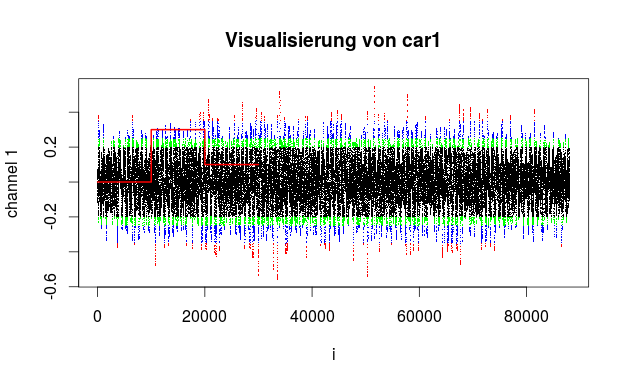
\includegraphics[width=512pt,height=280pt]{figures/bsp.png}
 	\caption{Ein Beispiel für ein Bild}
 	\label{bild:beispiel}
 \end{figure}
 
 
\section{Quellcode}

Quellcode wird automatisch (mit der Möglichkeit die Sprache anzugeben) formatiert und in das Listings-Verzeichnis gegeben:

\subsection{Java-Code}

\begin{lstlisting}[style=Java, caption={Java-Beispiel}, captionpos=b]
int i = 1;
float f = 2;
System.out.printf("Int-Z %d Float-Z: 52f",i ,f );
\end{lstlisting} 


\subsection{Python-Code}
 
\begin{lstlisting}[style=Python, caption={Python-Beispiel}, captionpos=b]
#Hier ein kleines Beispiel in Python
lower = 0
upper = 10
for i in range(lower,upper):
print(i)
\end{lstlisting} 


\subsection{Lesen von Dateien}
 
Es kann auch direkt von Dateien gelesen werden:

\lstinputlisting[style=Java, label={java_bsp}, caption={Java-Beispiel von Datei}, captionpos=b]{sourcecode/First.java}
 
\section{Referenzen}
			
Beispiele für die Verwendung von Referenzen: 

\begin{itemize}
	\item Wie in Tabelle ~\ref{tabelle:test} ersichtlich... 
	\item Wir sind im Kapitel ~\ref{chap:bsp}
	\item In Zeile 2 im Listing ~\ref{java_bsp} 
\end{itemize}


\section{Zitate}


Hier das Zitat eines Buches: \cite{couper2001} Wird alles automatisch mit  bibtex erledigt. % Einfach auskommentieren für die tatsächliche Arbeit


\appendix                       %% closes main document, appendix follows until end; only available in book-classes

\addpart*{Appendix}             %% adding Appendix to tableofcontents



\listoftables
\listoffigures
\lstlistoflistings
\nocite{*} %Es werden auf nicht referenzierte Literaturstellen aufgelistet
\bibliography{references}

\end{document}
